% The article, prepared for submission to the Journal of the Association for
% Information Science and Technology (JASIST, Wiley). Every number in it
% comes from a generated fragment (*.gen.tex, written by cmd/bench,
% cmd/compare, cmd/diagnose, cmd/coverage, cmd/result, cmd/cost, cmd/sweep);
% none is typed by hand. A \newcommand that is renamed, dropped or never
% generated shows up as a build failure here instead of as a stale number in
% a table nobody re-checked.
%
% Each section lives in its own .tex file next to this one; this file
% assembles them. The former appendix is built separately as
% supplement.tex (JASIST counts supplemental material outside the word
% limit and asks for it as a separate file).
%
% JASIST requirements this file implements (abbreviated author guidelines,
% August 2021, and the journal's "for authors" page):
%   - APA style citations and reference list      -> apacite
%   - abstract of at most 200 words, then keywords
%   - title page with affiliations, addresses, e-mail and corresponding author
%   - single or 1.5 line spacing                   -> single
%   - figures and tables after the paragraph that first mentions them -> [H]
%   - data availability, conflict of interest and funding statements
\documentclass[11pt]{article}
\usepackage[a4paper,margin=2.5cm]{geometry}
\usepackage[T1]{fontenc}
\usepackage[utf8]{inputenc}
\usepackage{microtype}
\usepackage{amsmath}
\usepackage{booktabs}
\usepackage{graphicx}
\usepackage{caption}
\usepackage{float}
\usepackage{tikz}
\usepackage{pgfplots}
\pgfplotsset{compat=1.18}
% APA 7 style references with natbib-compatible \citep / \citet commands.
\usepackage[natbibapa]{apacite}
\usepackage[hidelinks]{hyperref}

% Shared TikZ styles so that every architecture diagram uses the same visual
% vocabulary: grey = input/output text, blue = retrieval components, teal =
% storage, orange = LLM calls, yellow diamonds = decisions.
\usetikzlibrary{arrows.meta,positioning,shapes.geometric,fit,calc}
\tikzset{
  comp/.style={draw=black!60, rounded corners=2pt, minimum height=6.5mm,
               minimum width=15mm, align=center, font=\small, inner sep=3pt},
  q/.style={comp, fill=black!8},
  ret/.style={comp, fill=blue!12},
  store/.style={comp, cylinder, shape border rotate=90, aspect=0.12,
                fill=teal!15, minimum height=9mm},
  llm/.style={comp, fill=orange!22},
  ans/.style={comp, fill=green!15},
  dec/.style={draw=black!60, diamond, aspect=2.2, fill=yellow!25,
              align=center, font=\small, inner sep=1pt},
  doc/.style={comp, fill=violet!10, minimum width=12mm},
  arr/.style={-{Stealth[length=2mm]}, semithick},
  lbl/.style={font=\scriptsize, align=center}
}


% JASIST: "Figures and tables should be positioned in the manuscript after
% the paragraph in which they are first mentioned." [H] puts every float
% exactly where it stands in the source.
\floatplacement{figure}{H}
\floatplacement{table}{H}

% Fragments are input only when they exist, so the skeleton still builds
% while a run is half finished. A table that references a command from a
% fragment that is missing WILL fail, which is the intended signal.
\newcommand{\useresults}[1]{\IfFileExists{#1.gen.tex}{\input{#1.gen.tex}}{}}
% fragments.tex lists every *.gen.tex present; regenerate it with:
%   ls *.gen.tex | sed "s/\\.gen\\.tex$//" | awk '{print "\\useresults{" $0 "}"}' > fragments.tex
\useresults{adaptive-2wiki}
\useresults{adaptive-hotpotqa}
\useresults{adaptive-musique}
\useresults{adaptive-nq}
\useresults{adaptive-triviaqa}
\useresults{bm25-2wiki}
\useresults{bm25-hotpotqa}
\useresults{bm25-musique}
\useresults{bm25-nq}
\useresults{bm25-triviaqa}
\useresults{cascade-2wiki}
\useresults{cascade-hotpotqa}
\useresults{cascade-hybrid-2wiki}
\useresults{cascade-hybrid-hotpotqa}
\useresults{cascade-hybrid-musique}
\useresults{cascade-hybrid-nq}
\useresults{cascade-hybrid-triviaqa}
\useresults{cascade-llama-2wiki}
\useresults{cascade-llama-hotpotqa}
\useresults{cascade-llama-musique}
\useresults{cascade-llama-nq}
\useresults{cascade-llama-triviaqa}
\useresults{cascade-lp-2wiki}
\useresults{cascade-lp-hotpotqa}
\useresults{cascade-lp-musique}
\useresults{cascade-lp-nq}
\useresults{cascade-lp-triviaqa}
\useresults{cascade-musique}
\useresults{cascade-naive-2wiki}
\useresults{cascade-naive-hotpotqa}
\useresults{cascade-naive-musique}
\useresults{cascade-naive-nq}
\useresults{cascade-naive-triviaqa}
\useresults{cascade-nq}
\useresults{cascade-rr-2wiki}
\useresults{cascade-rr-hotpotqa}
\useresults{cascade-rr-musique}
\useresults{cascade-rr-nq}
\useresults{cascade-rr-triviaqa}
\useresults{cascade-triviaqa}
\useresults{closedbook-2wiki}
\useresults{closedbook-hotpotqa}
\useresults{closedbook-llama-2wiki}
\useresults{closedbook-llama-hotpotqa}
\useresults{closedbook-llama-musique}
\useresults{closedbook-llama-nq}
\useresults{closedbook-llama-triviaqa}
\useresults{closedbook-musique}
\useresults{closedbook-nq}
\useresults{closedbook-triviaqa}
\useresults{cmp-cascade-cascade-lp-2wiki}
\useresults{cmp-cascade-cascade-lp-hotpotqa}
\useresults{cmp-cascade-cascade-lp-musique}
\useresults{cmp-cascade-cascade-lp-nq}
\useresults{cmp-cascade-cascade-lp-triviaqa}
\useresults{cmp-cascade-hybrid-cascade-2wiki}
\useresults{cmp-cascade-hybrid-cascade-hotpotqa}
\useresults{cmp-cascade-hybrid-cascade-musique}
\useresults{cmp-cascade-hybrid-cascade-nq}
\useresults{cmp-cascade-hybrid-cascade-triviaqa}
\useresults{cmp-cascade-naive-cascade-2wiki}
\useresults{cmp-cascade-naive-cascade-hotpotqa}
\useresults{cmp-cascade-naive-cascade-musique}
\useresults{cmp-cascade-naive-cascade-nq}
\useresults{cmp-cascade-naive-cascade-triviaqa}
\useresults{cmp-cascade-rr-cascade-2wiki}
\useresults{cmp-cascade-rr-cascade-hotpotqa}
\useresults{cmp-cascade-rr-cascade-musique}
\useresults{cmp-cascade-rr-cascade-nq}
\useresults{cmp-cascade-rr-cascade-triviaqa}
\useresults{cmp-closedbook-naive-2wiki}
\useresults{cmp-closedbook-naive-hotpotqa}
\useresults{cmp-closedbook-naive-llama-2wiki}
\useresults{cmp-closedbook-naive-llama-hotpotqa}
\useresults{cmp-closedbook-naive-llama-musique}
\useresults{cmp-closedbook-naive-llama-nq}
\useresults{cmp-closedbook-naive-llama-triviaqa}
\useresults{cmp-closedbook-naive-musique}
\useresults{cmp-closedbook-naive-nq}
\useresults{cmp-closedbook-naive-triviaqa}
\useresults{cmp-fused-cascade-2wiki}
\useresults{cmp-fused-cascade-hotpotqa}
\useresults{cmp-fused-cascade-llama-2wiki}
\useresults{cmp-fused-cascade-llama-hotpotqa}
\useresults{cmp-fused-cascade-llama-musique}
\useresults{cmp-fused-cascade-llama-nq}
\useresults{cmp-fused-cascade-llama-triviaqa}
\useresults{cmp-fused-cascade-musique}
\useresults{cmp-fused-cascade-nq}
\useresults{cmp-fused-cascade-triviaqa}
\useresults{cmp-ircot-adaptive-2wiki}
\useresults{cmp-ircot-adaptive-hotpotqa}
\useresults{cmp-ircot-adaptive-musique}
\useresults{cmp-ircot-adaptive-nq}
\useresults{cmp-ircot-adaptive-triviaqa}
\useresults{cmp-ircot-ircot1-2wiki}
\useresults{cmp-ircot-ircot1-hotpotqa}
\useresults{cmp-ircot-ircot1-musique}
\useresults{cmp-ircot-ircot1-nq}
\useresults{cmp-ircot-ircot1-triviaqa}
\useresults{cmp-ircot1-cascade-2wiki}
\useresults{cmp-ircot1-cascade-hotpotqa}
\useresults{cmp-ircot1-cascade-musique}
\useresults{cmp-ircot1-cascade-nq}
\useresults{cmp-ircot1-cascade-triviaqa}
\useresults{cmp-naive-adaptive-2wiki}
\useresults{cmp-naive-adaptive-hotpotqa}
\useresults{cmp-naive-adaptive-musique}
\useresults{cmp-naive-adaptive-nq}
\useresults{cmp-naive-adaptive-triviaqa}
\useresults{cmp-naive-bm25-2wiki}
\useresults{cmp-naive-bm25-hotpotqa}
\useresults{cmp-naive-bm25-musique}
\useresults{cmp-naive-bm25-nq}
\useresults{cmp-naive-bm25-triviaqa}
\useresults{cmp-naive-cascade-2wiki}
\useresults{cmp-naive-cascade-hotpotqa}
\useresults{cmp-naive-cascade-llama-2wiki}
\useresults{cmp-naive-cascade-llama-hotpotqa}
\useresults{cmp-naive-cascade-llama-musique}
\useresults{cmp-naive-cascade-llama-nq}
\useresults{cmp-naive-cascade-llama-triviaqa}
\useresults{cmp-naive-cascade-lp-2wiki}
\useresults{cmp-naive-cascade-lp-hotpotqa}
\useresults{cmp-naive-cascade-lp-musique}
\useresults{cmp-naive-cascade-lp-nq}
\useresults{cmp-naive-cascade-lp-triviaqa}
\useresults{cmp-naive-cascade-musique}
\useresults{cmp-naive-cascade-nq}
\useresults{cmp-naive-cascade-triviaqa}
\useresults{cmp-naive-hybrid-2wiki}
\useresults{cmp-naive-hybrid-hotpotqa}
\useresults{cmp-naive-hybrid-musique}
\useresults{cmp-naive-hybrid-nq}
\useresults{cmp-naive-hybrid-triviaqa}
\useresults{cmp-naive-hyde-2wiki}
\useresults{cmp-naive-hyde-hotpotqa}
\useresults{cmp-naive-hyde-musique}
\useresults{cmp-naive-hyde-nq}
\useresults{cmp-naive-hyde-triviaqa}
\useresults{cmp-naive-rerank-2wiki}
\useresults{cmp-naive-rerank-hotpotqa}
\useresults{cmp-naive-rerank-llama-2wiki}
\useresults{cmp-naive-rerank-llama-hotpotqa}
\useresults{cmp-naive-rerank-llama-musique}
\useresults{cmp-naive-rerank-llama-nq}
\useresults{cmp-naive-rerank-llama-triviaqa}
\useresults{cmp-naive-rerank-musique}
\useresults{cmp-naive-rerank-nq}
\useresults{cmp-naive-rerank-triviaqa}
\useresults{cmp-naive10-crag10-2wiki}
\useresults{cmp-naive10-crag10-hotpotqa}
\useresults{cmp-naive10-crag10-musique}
\useresults{cmp-naive10-ircot-2wiki}
\useresults{cmp-naive10-ircot-hotpotqa}
\useresults{cmp-naive10-ircot-musique}
\useresults{cmp-naive10-ircot1-2wiki}
\useresults{cmp-naive10-ircot1-hotpotqa}
\useresults{cmp-naive10-ircot1-musique}
\useresults{cmp-naive12-neighbour-2wiki}
\useresults{cmp-naive12-neighbour-hotpotqa}
\useresults{cmp-naive12-neighbour-musique}
\useresults{cmp-rerank-cascade-2wiki}
\useresults{cmp-rerank-cascade-hotpotqa}
\useresults{cmp-rerank-cascade-llama-2wiki}
\useresults{cmp-rerank-cascade-llama-hotpotqa}
\useresults{cmp-rerank-cascade-llama-musique}
\useresults{cmp-rerank-cascade-llama-nq}
\useresults{cmp-rerank-cascade-llama-triviaqa}
\useresults{cmp-rerank-cascade-lp-2wiki}
\useresults{cmp-rerank-cascade-lp-hotpotqa}
\useresults{cmp-rerank-cascade-lp-musique}
\useresults{cmp-rerank-cascade-lp-nq}
\useresults{cmp-rerank-cascade-lp-triviaqa}
\useresults{cmp-rerank-cascade-musique}
\useresults{cmp-rerank-cascade-nq}
\useresults{cmp-rerank-cascade-triviaqa}
\useresults{cmp-rerank-fused-2wiki}
\useresults{cmp-rerank-fused-hotpotqa}
\useresults{cmp-rerank-fused-llama-2wiki}
\useresults{cmp-rerank-fused-llama-hotpotqa}
\useresults{cmp-rerank-fused-llama-musique}
\useresults{cmp-rerank-fused-llama-nq}
\useresults{cmp-rerank-fused-llama-triviaqa}
\useresults{cmp-rerank-fused-musique}
\useresults{cmp-rerank-fused-nq}
\useresults{cmp-rerank-fused-triviaqa}
\useresults{cost}
\useresults{coverage-2wiki}
\useresults{coverage-hotpotqa}
\useresults{coverage-musique}
\useresults{crag-2wiki}
\useresults{crag-hotpotqa}
\useresults{crag-musique}
\useresults{crag-nq}
\useresults{crag-triviaqa}
\useresults{crag10-2wiki}
\useresults{crag10-hotpotqa}
\useresults{crag10-musique}
\useresults{diagnosis-2wiki}
\useresults{diagnosis-hotpotqa}
\useresults{diagnosis-musique}
\useresults{fused-2wiki}
\useresults{fused-hotpotqa}
\useresults{fused-llama-2wiki}
\useresults{fused-llama-hotpotqa}
\useresults{fused-llama-musique}
\useresults{fused-llama-nq}
\useresults{fused-llama-triviaqa}
\useresults{fused-musique}
\useresults{fused-nq}
\useresults{fused-triviaqa}
\useresults{hybrid-2wiki}
\useresults{hybrid-hotpotqa}
\useresults{hybrid-musique}
\useresults{hybrid-nq}
\useresults{hybrid-triviaqa}
\useresults{hyde-2wiki}
\useresults{hyde-hotpotqa}
\useresults{hyde-musique}
\useresults{hyde-nq}
\useresults{hyde-triviaqa}
\useresults{ircot-2wiki}
\useresults{ircot-hotpotqa}
\useresults{ircot-musique}
\useresults{ircot-nq}
\useresults{ircot-triviaqa}
\useresults{ircot1-2wiki}
\useresults{ircot1-hotpotqa}
\useresults{ircot1-musique}
\useresults{ircot1-nq}
\useresults{ircot1-triviaqa}
\useresults{naive-2wiki}
\useresults{naive-hotpotqa}
\useresults{naive-llama-2wiki}
\useresults{naive-llama-hotpotqa}
\useresults{naive-llama-musique}
\useresults{naive-llama-nq}
\useresults{naive-llama-triviaqa}
\useresults{naive-musique}
\useresults{naive-nq}
\useresults{naive-triviaqa}
\useresults{naive10-2wiki}
\useresults{naive10-hotpotqa}
\useresults{naive10-musique}
\useresults{naive12-2wiki}
\useresults{naive12-hotpotqa}
\useresults{naive12-musique}
\useresults{neighbour-2wiki}
\useresults{neighbour-hotpotqa}
\useresults{neighbour-musique}
\useresults{rerank-2wiki}
\useresults{rerank-hotpotqa}
\useresults{rerank-llama-2wiki}
\useresults{rerank-llama-hotpotqa}
\useresults{rerank-llama-musique}
\useresults{rerank-llama-nq}
\useresults{rerank-llama-triviaqa}
\useresults{rerank-musique}
\useresults{rerank-nq}
\useresults{rerank-triviaqa}
\useresults{result-llama}
\useresults{result-lp}
\useresults{result}
\useresults{sweep}


\title{CascadeRAG: Abstention-Triggered Escalation\\
that Outperforms Costlier Retrieval-Augmented Generation\\
Architectures at a Fraction of their Cost}
\author{Miko{\l}aj Semeniuk$^{1,*}$ \and Agnieszka Jastrz{\k{e}}bska$^{1}$\\[2ex]
\normalsize $^{1}$Faculty of Mathematics and Information Science,
Warsaw University of Technology,\\
\normalsize Koszykowa 75, 00-662 Warsaw, Poland\\[1ex]
\normalsize $^{*}$Corresponding author: \href{mailto:m.semeniuk@icloud.com}{m.semeniuk@icloud.com},
ORCID \href{https://orcid.org/0009-0001-2247-2004}{0009-0001-2247-2004}}
\date{}

\begin{document}

\maketitle

% JASIST: an informative abstract of at most 200 words.
\begin{abstract}
Retrieval-Augmented Generation (RAG) grounds a language model's answers in
an external document collection, and many architectural refinements
compete for a place in practical systems. Their published evaluations are
rarely comparable, because each uses its own corpus, retriever, generator,
and context budget. We present a controlled comparison of thirteen RAG
architectures on a single stack (one 21-million-passage corpus, one
embedding model, one generator, one prompt) over five question sets and
more than 37{,}000 questions, with paired significance tests under
multiplicity control, budget-matched controls, abstention measured
separately from error, and retrieval read against the measured ceiling the
corpus imposes. No refinement is universally safe: cross-encoder reranking
gains $+0.051$ Exact Match on one question set and loses $0.100$ on
another. A per-question diagnosis of why retrieval fails explains these
reversals and yields a novel design, CascadeRAG: retrieve with a fusion of
dense, lexical, and cross-encoder rankings, and escalate to a costlier
strategy only when the reader itself declines to answer, a posterior signal
that is provably lossless under Exact Match. Across \ResultPairs{} paired
comparisons CascadeRAG wins \ResultWins{}, loses \ResultLosses{}, and ties
\ResultTies{}, at 1.16--1.58 generator calls per question against 2.3--3.0
for iterative and corrective methods, and replicates under a second
generator.
\end{abstract}

\noindent\textbf{Keywords:} retrieval-augmented generation; large language
models; question answering; information retrieval; evaluation methodology;
cascade architectures

\section{Introduction}
\label{sec:introduction}

Large language models answer factual questions from knowledge stored in their
weights, and that knowledge is incomplete, frozen at training time, and
expensive to change. Retrieval-Augmented Generation
(RAG)~\citep{lewis2020rag} addresses all three problems at once: instead of
asking the model to remember, the system searches an external document
collection for passages relevant to the question and places them in the
model's context, so that the model reads rather than recalls. The technique
has become the default way of grounding language models in private,
fresh, or specialised document collections, and a large family of
architectural refinements has grown around it: lexical--dense hybrid
retrieval, cross-encoder reranking, hypothetical document embeddings,
corrective retrieval, iterative retrieval interleaved with reasoning, and
routers that pick a strategy per question.

The difficulty, for anyone who has to choose among these architectures, is
that each refinement is usually evaluated by its authors on their own stack
--- their own corpus, chunking, retriever, generator, and prompts --- and
against a small set of baselines. Published numbers are therefore rarely
comparable across papers, and improvements measured on one stack routinely
fail to transfer to another. Worse, our measurements show that the
refinements are not uniformly safe: the strongest single retrieval
improvement we measure, cross-encoder reranking, gains
$+0.051$ Exact Match over the standard baseline on HotpotQA and
\emph{loses} $-0.100$ on NaturalQuestions --- a catastrophic regression that
a single-benchmark evaluation would never reveal. Practitioners deploying
RAG face a menu of architectures whose relative merits depend on the
question distribution in ways the literature does not document.

This article makes three contributions.

\begin{enumerate}
\item \textbf{A controlled, statistically grounded comparison of thirteen
RAG architectures.} Every architecture is evaluated on the same 21-million-passage
Wikipedia corpus, the same embedding model, the same vector database, the
same generator, and the same answer prompt, over five question sets
(NaturalQuestions, TriviaQA, HotpotQA, 2WikiMultihopQA, MuSiQue) totalling
more than 37{,}000 questions --- so that the only difference between two rows of
a results table is the architecture itself. Differences are tested with
paired statistics (McNemar's test on Exact Match, Wilcoxon signed-rank on
continuous metrics) under a Holm correction, and every retrieval figure is
reported against the ceiling the corpus imposes, which we measure. Budget-matched
controls separate ``a better architecture'' from ``more text in the
context'', and abstention is measured separately from error, which reverses
one published-style conclusion (Section~\ref{sec:results}).

\item \textbf{A diagnosis of \emph{why} retrieval fails.} Aggregate recall
cannot distinguish failure causes that call for entirely different fixes. We
classify the baseline's retrieval failures into five causes --- wrong slice
of the right article, right article ranked too low, article unreachable by
the question's own vocabulary, no gold article stating the answer, and
article absent from the corpus --- and show that the distribution of causes,
not any aggregate score, predicts which architectural refinement pays off
on which question set.

\item \textbf{CascadeRAG, a novel cascade architecture constructed based
on lessons learned from the conducted studies.} CascadeRAG combines a fused first stage --- dense, lexical, and cross-encoder rankings
merged by Reciprocal Rank Fusion, which avoids the reranker's collapse
while keeping most of its gain --- with \emph{abstention-triggered
escalation}: only when the reader itself declines to answer, having seen
the retrieved passages, is the question handed to a more expensive
strategy. The trigger is a \emph{posterior} signal, unlike routers that
predict difficulty from the question alone, and it is \emph{lossless} under
Exact Match: across all 887{,}917 (question, architecture) pairs measured
here, no abstention ever scores Exact Match~1, so escalation cannot discard
a correct answer. Against every baseline on every question set CascadeRAG
wins \ResultWins{} of \ResultPairs{} paired comparisons, loses
\ResultLosses{}, and ties \ResultTies{}, at 1.16--1.58 generator calls per
question --- against 2.3 for iterative retrieval and 3.0 for corrective
RAG. The result replicates under a second, unrelated generator.
\end{enumerate}

\begin{figure}[t]
\centering
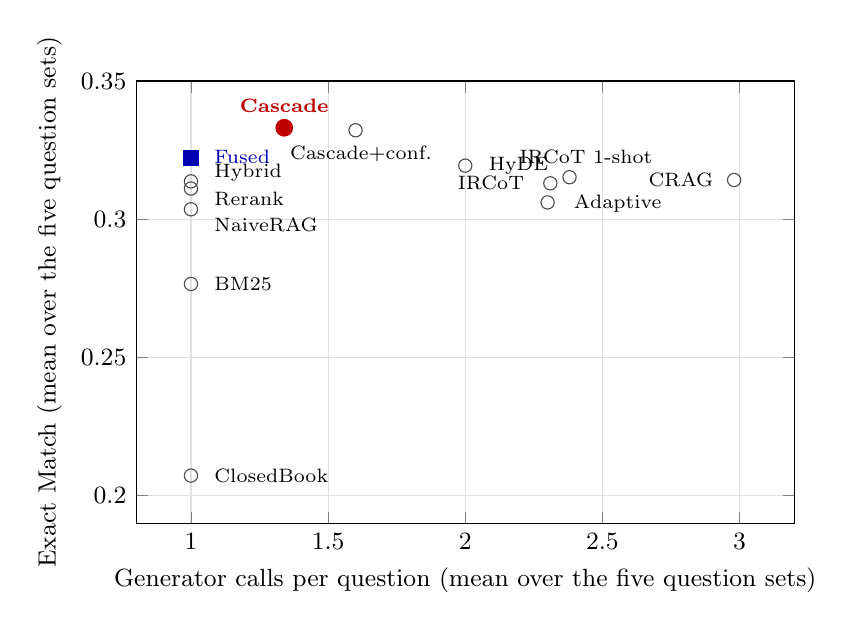
\begin{tikzpicture}
\begin{axis}[
    width=0.82\textwidth, height=7.2cm,
    xlabel={Generator calls per question (mean over the five question sets)},
    ylabel={Exact Match (mean over the five question sets)},
    xmin=0.8, xmax=3.2, ymin=0.19, ymax=0.35,
    grid=major, grid style={black!12},
    tick label style={font=\small}, label style={font=\small},
    every node near coord/.append style={font=\scriptsize}
]
% Means computed from the per-set generated fragments (paper/*.gen.tex);
% per-set values and significance tests are in Section 7.
\addplot[only marks, mark=o, mark size=2.4pt, black!70] coordinates {
    (1.00,0.2073) (1.00,0.2766) (1.00,0.3036) (1.00,0.3137) (1.00,0.3111)
    (2.00,0.3194) (2.98,0.3142) (2.31,0.3130) (2.38,0.3152) (2.30,0.3061)
    (1.60,0.3322)
};
\addplot[only marks, mark=square*, mark size=2.6pt, blue!70!black] coordinates {
    (1.00,0.3222)
};
\addplot[only marks, mark=*, mark size=3pt, red!75!black] coordinates {
    (1.34,0.3331)
};
\node[font=\scriptsize, anchor=west] at (axis cs:1.05,0.2073) {ClosedBook};
\node[font=\scriptsize, anchor=west] at (axis cs:1.05,0.2766) {BM25};
\node[font=\scriptsize, anchor=west] at (axis cs:1.05,0.2980) {NaiveRAG};
\node[font=\scriptsize, anchor=west] at (axis cs:1.05,0.3170) {Hybrid};
\node[font=\scriptsize, anchor=west] at (axis cs:1.05,0.3075) {Rerank};
\node[font=\scriptsize, anchor=west, blue!70!black] at (axis cs:1.05,0.3225) {Fused};
\node[font=\scriptsize, anchor=west] at (axis cs:2.05,0.3194) {HyDE};
\node[font=\scriptsize, anchor=east] at (axis cs:2.94,0.3142) {CRAG};
\node[font=\scriptsize, anchor=east] at (axis cs:2.25,0.3130) {IRCoT};
\node[font=\scriptsize, anchor=south] at (axis cs:2.44,0.3165) {IRCoT 1-shot};
\node[font=\scriptsize, anchor=west] at (axis cs:2.36,0.3055) {Adaptive};
\node[font=\scriptsize, anchor=south, red!75!black] at (axis cs:1.34,0.3350) {\textbf{Cascade}};
\node[font=\scriptsize, anchor=north] at (axis cs:1.62,0.3300) {Cascade+conf.};
\end{axis}
\end{tikzpicture}
\caption{Answer quality against generator cost for every architecture
measured in this article, averaged over the five question sets. The
proposed cascade (red) reaches the highest mean Exact Match at a fraction
of the cost of the iterative and corrective methods; its first stage alone
(Fused, blue) already dominates the single-call architectures. Per-set results,
in which no single architecture wins everywhere, are analysed in
Section~\ref{sec:results}.}
\label{fig:pareto}
\end{figure}

A fourth, methodological contribution runs through the article: every
number reported here --- every cell of every table, including those in this
sentence --- is generated by the benchmark code directly from the
per-question output files and imported into the manuscript as a named
macro, so no figure can drift from the experiment that produced it. The
benchmark, the analysis tools, and the manuscript build are one
reproducible pipeline, which we publicly share together with the per-question
logs.\footnote{\url{https://github.com/mikolajsemeniuk/ragbench}}

The article is organised for two audiences. Sections~\ref{sec:background}
and~\ref{sec:architectures} are self-contained: they explain how RAG works
--- embeddings, similarity search, vector databases, and why retrieval is
preferred to retraining --- and then describe each compared architecture
with a uniform template and diagram, so that a reader new to the area can
follow the rest. Sections~\ref{sec:cascade}--\ref{sec:results} present the
proposed architecture, the experimental protocol, and the results;
Section~\ref{sec:discussion} distils practical guidance;
Section~\ref{sec:limitations} states limitations.

\section{Background: how retrieval-augmented generation works}
\label{sec:background}

This section is a self-contained primer. Readers familiar with dense
retrieval and RAG can skip to Section~\ref{sec:related}; every concept
introduced here is used later to explain a measured result.

\subsection{The knowledge problem, and why not simply retrain the model}
\label{sec:why-rag}

A large language model stores what it knows in its
weights~\cite{brown2020gpt3,petroni2019lmkb} --- so-called
\emph{parametric} knowledge, acquired once, during training. Three
consequences follow. First, the knowledge is \emph{frozen}: a model trained
in 2024 knows nothing that happened afterwards. Second, it is
\emph{incomplete and unreliable}: how much a model retains depends on how
often it saw a fact~\cite{roberts2020knowledge,kandpal2023longtail} ---
popular facts appear thousands of times where rare facts appear once or
never~\cite{mallen2023popqa} --- and when asked about the latter it tends
to produce fluent, plausible, wrong answers ---
hallucinations~\cite{ji2023hallucination,zhang2023sirens}. Third, it is
\emph{closed}: an
organisation's internal documentation, product catalogue, or case history
was never in the training data at all.

The obvious remedy --- continue training the model on the missing documents
--- is rarely practical. Full retraining of even a mid-sized model costs
GPU-months; parameter-efficient fine-tuning~\cite{hu2022lora} is cheaper
but must be repeated every time the documents change, offers no
attribution (the model still cannot say \emph{where} an answer came
from), and injects new factual knowledge less reliably than simply
retrieving it~\cite{ovadia2024finetuning}. Retrieval-Augmented
Generation~\cite{lewis2020rag} sidesteps the problem: the documents stay
outside the model, in a searchable index that can be updated by inserting
or deleting a record, and at question time the system retrieves the few
passages most relevant to the question and prepends them to the model's
prompt. The model's job shrinks from \emph{recalling} the fact to
\emph{reading} it. Updating knowledge becomes a database operation rather than
a training run; a company can place its private business context into the
index without any of it entering the model's weights; and every answer can
cite the passages it was read from.

\subsection{Embeddings and cosine similarity}
\label{sec:embeddings}

The search step must match a question to passages by \emph{meaning}, not
just by shared words --- ``Where did the director of Beat Girl die?'' shares
almost no vocabulary with the encyclopedia paragraph that answers it. The
standard tool is the \emph{text embedding}: a neural network (the
\emph{embedding model} or \emph{encoder}, typically a Transformer
encoder~\cite{vaswani2017attention,devlin2019bert}) that maps a piece of
text to a vector of a few hundred real numbers, trained so that texts
with similar meaning land close together in that vector
space~\cite{reimers2019sbert}.

Closeness is measured by \emph{cosine similarity}: the cosine of the angle
between two vectors, which is $1$ for parallel vectors, $0$ for orthogonal
ones, and $-1$ for opposite ones. For vectors $\mathbf{a}$ and $\mathbf{b}$,
\begin{equation}
\cos(\mathbf{a},\mathbf{b})
  = \frac{\mathbf{a}\cdot\mathbf{b}}{\lVert\mathbf{a}\rVert\,\lVert\mathbf{b}\rVert}
  = \frac{\sum_i a_i b_i}{\sqrt{\sum_i a_i^2}\sqrt{\sum_i b_i^2}}.
\end{equation}
A toy example with three dimensions makes the mechanics concrete. Suppose an
encoder mapped three texts as follows:
\begin{center}
\small
\begin{tabular}{lr}
\toprule
Text & Vector \\
\midrule
``Who directed Beat Girl?'' & $(0.9,\; 0.4,\; 0.1)$ \\
``Beat Girl is a 1960 film directed by Edmond T.\ Gr\'eville.'' & $(0.8,\; 0.5,\; 0.2)$ \\
``The recipe calls for two eggs and a cup of flour.'' & $(0.1,\; 0.2,\; 0.9)$ \\
\bottomrule
\end{tabular}
\end{center}
The question and the film passage give
$\cos = (0.72+0.20+0.02)/(1.0\cdot0.97) \approx 0.97$; the question and the
recipe give $\cos \approx 0.35$. The film passage is retrieved. Real
encoders behave the same way in 768 dimensions instead of three.

Two properties of embeddings matter for the results in this article. First,
an embedding is a \emph{lossy compression}: 768 numbers cannot preserve
everything in a hundred-word passage, and what the compression loses first
is rare surface forms --- exact titles, names, codes. A question that names
its target verbatim can therefore still miss it in embedding space, which
is precisely the failure that lexical search repairs
(Section~\ref{sec:arch-hybrid}). Second, some encoders are trained
\emph{asymmetrically}: the query is expected to carry a short instruction
prefix (e.g.\ \texttt{query:}~\ldots) that the passage side does not.
Ignoring the convention silently degrades retrieval; we verify the
convention for our encoder empirically (Section~\ref{sec:setup}).

\subsection{Embedding models and cross-encoders}
\label{sec:encoders}

The encoder used for search is a \emph{bi-encoder}: it embeds the question
and each passage \emph{separately}, and their relevance is the similarity
of the two vectors. This is what makes web-scale search possible --- all
passage vectors are computed once, offline, and a question at query time is
embedded once and compared against millions of stored vectors in
milliseconds. The price is that the encoder never sees the question and the
passage \emph{together}, so it cannot model their interaction; it matches
what a question is \emph{about}.

A \emph{cross-encoder}~\cite{nogueira2019passage} reads the concatenated
(question, passage) pair through one network and outputs a relevance score.
Seeing both texts jointly, it can judge whether the passage actually
answers the question --- what the question is \emph{asking for} --- far
more precisely, but at the cost of one full network pass per pair, which
rules out scanning a corpus. The standard compromise is a two-stage
pipeline: a bi-encoder retrieves a shortlist of candidates, and the
cross-encoder reorders the shortlist (Section~\ref{sec:arch-rerank}). The
distinction between \emph{about} and \emph{asking for} is not cosmetic; it
produces the single largest failure we measure
(Section~\ref{sec:results-single}).

\subsection{Vector databases}
\label{sec:vectordb}

Storing millions of embedding vectors and answering ``which stored vectors
are most similar to this query vector'' is the job of a \emph{vector
database}. Comparing the query against every stored vector (exact search)
is linear in corpus size; even GPU-accelerated exact
search~\cite{johnson2019faiss} is a poor fit for serving interactive
queries at the 21-million-passage scale used here. Vector databases therefore build an
\emph{approximate nearest neighbour} (ANN) index --- most commonly a
Hierarchical Navigable Small World graph (HNSW)~\cite{malkov2020hnsw}, a
layered proximity graph walked greedily from an entry point towards the
query. The walk inspects a small fraction of the corpus and returns the
nearest vectors it visited, trading a tunable amount of recall for orders of
magnitude in speed; the size of the candidate list the walk keeps
(\texttt{ef}) controls that trade, and we report and fix it in our setup
because a benchmark that leaves it at an unknown default silently measures
the index rather than the architecture.

Alongside each vector, the database stores the passage text and its
identifier, so a search returns readable passages, ready to be placed in a
prompt. The same database can also host a \emph{sparse} (lexical) index, in
which a passage is represented by weighted term counts and matching is by
exact term overlap under BM25 scoring~\cite{robertson2009bm25} --- the
modern packaging of classical keyword search, and the complement to dense
retrieval used by the hybrid architectures below.

\subsection{The naive RAG pipeline}
\label{sec:naive-pipeline}

\begin{figure}[t]
\centering
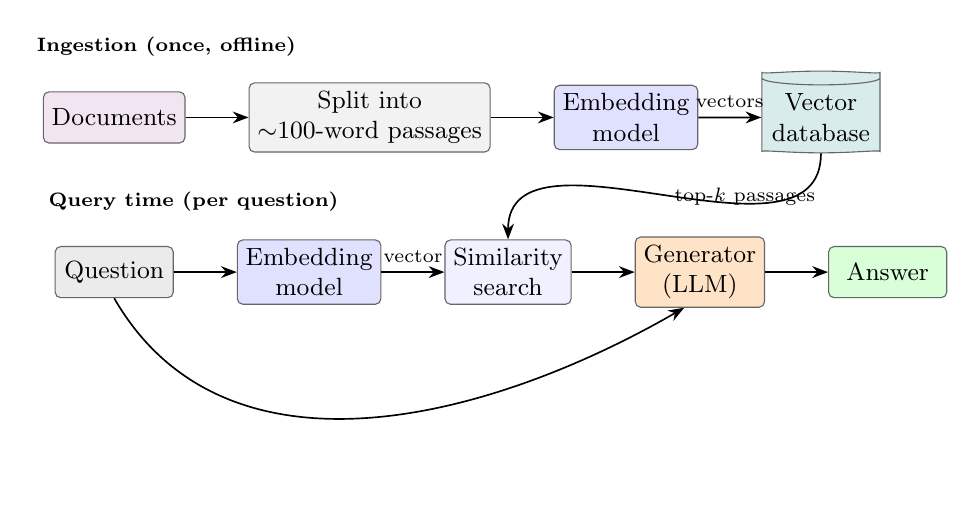
\begin{tikzpicture}[node distance=5mm and 8mm]
% Ingestion phase
\node[doc] (corpus) {Documents};
\node[comp, fill=black!5, right=of corpus] (chunk) {Split into\\$\sim$100-word passages};
\node[ret, right=of chunk] (encdoc) {Embedding\\model};
\node[store, right=of encdoc] (db) {Vector\\database};
\draw[arr] (corpus) -- (chunk);
\draw[arr] (chunk) -- (encdoc);
\draw[arr] (encdoc) -- node[lbl, above] {vectors} (db);
\node[lbl, anchor=west] at ($(corpus.west)+(-2mm,9mm)$) {\textbf{Ingestion (once, offline)}};
% Query phase
\node[q, below=13mm of corpus] (question) {Question};
\node[ret, right=of question] (encq) {Embedding\\model};
\node[comp, fill=blue!6, right=of encq] (search) {Similarity\\search};
\node[llm, right=of search] (gen) {Generator\\(LLM)};
\node[ans, right=of gen] (answer) {Answer};
\draw[arr] (question) -- (encq);
\draw[arr] (encq) -- node[lbl, above] {vector} (search);
\draw[arr] (db.south) to[out=-90,in=90] node[lbl, right] {top-$k$ passages} (search.north);
\draw[arr] (search) -- (gen);
\draw[arr] (gen) -- (answer);
\draw[arr] (question.south) to[out=-60,in=-150] ($(gen.south)+(-2mm,0)$);
\node[lbl, anchor=west] at ($(question.west)+(-2mm,9mm)$) {\textbf{Query time (per question)}};
\end{tikzpicture}
\caption{The naive RAG pipeline. Offline, the document collection is split
into passages, embedded, and stored in a vector database. At query time the
question is embedded with the same model, the $k$ most similar passages are
retrieved, and the generator answers from the question plus those passages.
Every architecture in this article is a modification of one or more blocks
of this pipeline.}
\label{fig:naive-pipeline}
\end{figure}

Figure~\ref{fig:naive-pipeline} assembles the components into the baseline
architecture that every refinement modifies. Offline, the collection is
split into passages of roughly one hundred words --- small enough that a
retrieved passage is mostly about one thing, large enough to carry a fact
in context --- and each passage is embedded and stored. At query time, the
question is embedded, the $k$ most similar passages are retrieved (here
$k=5$), and the generator receives a prompt of the form ``Answer the
question based on the given documents\ldots'' followed by the passages and
the question.

This pipeline can fail in one of a few ways: the passage that answers the
question is in the corpus but ranked below the top~$k$; it is unreachable because the question's own words are
too far from it in embedding space; the right article was found but the
wrong hundred-word slice of it was taken; or the answer simply is not in
the corpus. Which of these dominates depends on the question distribution,
and measuring that split --- rather than guessing it --- is what
Section~\ref{sec:results-diagnosis} contributes; the architectures of
Section~\ref{sec:architectures} are, in effect, one remedy per failure
mode. The generation side has failure modes of its own --- readers use
passages unevenly by position in the context~\cite{liu2024lost}, react
measurably to irrelevant passages~\cite{cuconasu2024noise}, and
engineering surveys catalogue further failure points across the
pipeline~\cite{barnett2024seven} --- but on this benchmark the bulk of
the measurable headroom sits in retrieval, which is where the diagnosis
looks.

\section{Related work}
\label{sec:related}

\paragraph{Retrieval-augmented generation.}
RAG was introduced as a trainable combination of a dense
retriever~\citep{karpukhin2020dpr} and a sequence-to-sequence
generator~\citep{lewis2020rag}, alongside a family of retrieval-augmented
language models that condition on retrieved text during pre-training or
decoding --- REALM~\citep{guu2020realm}, FiD~\citep{izacard2021fid},
RETRO~\citep{borgeaud2022retro}, $k$NN-LM~\citep{khandelwal2020knnlm}.
Contemporary practice replaces the trained combination with a frozen
instruction-following LLM reading retrieved passages in its
prompt~\citep{ram2023incontext,shi2024replug}, the form studied here. Surveys chart the field's rapid growth
and its progression from naive through advanced to modular
pipelines~\citep{gao2023ragsurvey} and, most recently, to agentic
systems~\citep{singh2025agenticrag}.

\paragraph{Retrieval-side refinements.}
Classical lexical scoring~\citep{robertson2009bm25} survives inside modern
stacks as the complement to dense retrieval, with Reciprocal Rank
Fusion~\citep{cormack2009rrf} the standard way to merge the two rankings.
Cross-encoder reranking~\citep{nogueira2019passage} re-scores a dense
shortlist with a jointly-encoded relevance model. These methods keep one
generator call per question and modify only which passages reach it.

\paragraph{Query-side refinements.}
HyDE~\citep{gao2022hyde} searches with a model-drafted hypothetical answer
passage instead of the question, bridging the vocabulary gap between
questions and encyclopedic text. IRCoT~\citep{trivedi2023ircot} interleaves
one sentence of chain-of-thought reasoning~\citep{wei2022cot} with one
retrieval per step, so that entities surfaced by reasoning become
retrievable queries --- the canonical mechanism for multi-hop questions,
related in spirit to acting-and-reasoning agents~\citep{yao2023react}.
Neighbouring iterative schemes decompose the question into explicit
sub-questions (Self-Ask~\citep{press2023selfask}), retrieve whenever the
model's next sentence is uncertain (FLARE~\citep{jiang2023flare}), or
alternate full generation and retrieval rounds
(Iter-RetGen~\citep{shao2023iterretgen}).

\paragraph{Self-assessing and adaptive systems.}
Self-RAG~\citep{asai2024selfrag} trains a model to emit reflection tokens
deciding when to retrieve and whether generations are supported. CRAG
\citep{yan2024crag} grades retrieved passages with a trained evaluator and
triggers corrective web search when the retrieval is judged poor.
Adaptive-RAG~\citep{jeong2024adaptiverag} trains a classifier that routes
each question to no-retrieval, single-step, or multi-step pipelines. All
three decide how much work a question needs; the cascade proposed here
differs in \emph{when} the decision is made --- after the reader has seen
the evidence (a posterior signal) rather than from the question alone (a
prior one) --- and in requiring no trained component at all.

\paragraph{Structure-augmented retrieval.}
GraphRAG~\citep{edge2024graphrag}, RAPTOR~\citep{sarthi2024raptor} and
HippoRAG~2~\citep{gutierrez2025hipporag2} preprocess the corpus into graphs,
trees, or memory structures. They occupy a different cost class --- their
indexing step itself involves large-scale LLM calls over the corpus --- and
systematic evaluation finds their advantage concentrated in query-focused
summarisation rather than factoid QA~\citep{han2025ragvsgraphrag}; we
therefore exclude them from a comparison whose corpus is 21M passages, and
note the exclusion as a limitation (see Section~\ref{sec:limitations}).

\paragraph{Benchmarks and evaluation.}
FlashRAG~\citep{jin2024flashrag} standardises datasets, corpora, and
reimplementations of a dozen RAG methods, and is the source of our corpus
and question sets; MultiHop-RAG~\citep{tang2024multihoprag} benchmarks
multi-hop retrieval specifically, BEIR~\citep{thakur2021beir} zero-shot
retrieval, and RGB~\citep{chen2024benchmarking} the generation step's
robustness to noisy passages; RAGAS~\citep{es2024ragas} offers
reference-free evaluation, and best-practice studies tune pipeline
components in isolation~\citep{wang2024bestpractices}. Our work differs
from toolkit
benchmarking in three ways: paired significance testing with multiplicity
control instead of point scores; measurement of the corpus-imposed recall
ceiling and of abstention as a behaviour distinct from error; and a
per-question failure diagnosis that connects each architecture's gain to
the failure mode it repairs.

\paragraph{Cascades (the new approach).}
Deferring expensive computation until a cheap stage proves insufficient has
a long history --- boosted detector cascades in
vision~\citep{viola2001cascade} and cascade ranking in
retrieval~\citep{wang2011cascade}. The architecture proposed here applies
the idea at the level of whole RAG strategies, with the reader's own
refusal as the deferral signal; to our knowledge the losslessness of that
trigger under span-level Exact Match has not previously been stated or
exploited.

\section{The architectures under study}
\label{sec:architectures}

We compare thirteen architectures: a no-retrieval bottom line, the naive
baseline at three context budgets, and nine refinements drawn from the
families of Section~\ref{sec:related}. Figure~\ref{fig:taxonomy} groups
them by the shape of their control flow, following the taxonomy of
\citet{jin2024flashrag}: \emph{sequential} architectures run the pipeline of
Figure~\ref{fig:naive-pipeline} once, changing only which passages reach
the generator; \emph{branching} architectures add a generation step before
retrieval; \emph{conditional} architectures inspect intermediate state and
choose among actions; \emph{iterative} architectures loop.
Table~\ref{tab:qualitative} summarises what each one changes and what it
costs. Each architecture below is described with the same template and names
the measured failure mode it targets (Section~\ref{sec:results-diagnosis}).

\begin{figure}
\centering
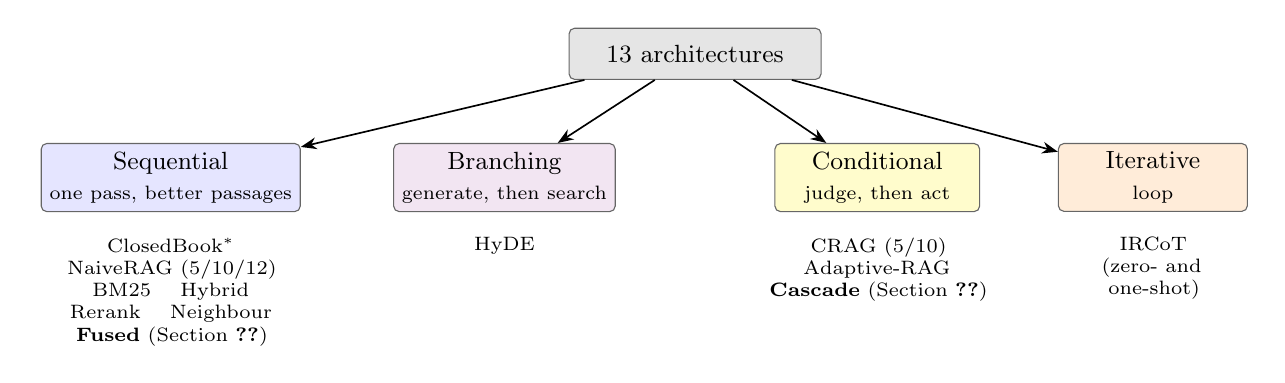
\begin{tikzpicture}[node distance=3mm and 5mm]
\node[comp, fill=black!10, minimum width=32mm] (root) {13 architectures};
\node[comp, fill=blue!10, below left=8mm and 34mm of root, minimum width=30mm] (seq) {Sequential\\ \scriptsize one pass, better passages};
\node[comp, fill=violet!10, below left=8mm and -6mm of root, minimum width=26mm] (bra) {Branching\\ \scriptsize generate, then search};
\node[comp, fill=yellow!20, below right=8mm and -6mm of root, minimum width=26mm] (con) {Conditional\\ \scriptsize judge, then act};
\node[comp, fill=orange!15, below right=8mm and 30mm of root, minimum width=24mm] (ite) {Iterative\\ \scriptsize loop};
\draw[arr] (root) -- (seq); \draw[arr] (root) -- (bra);
\draw[arr] (root) -- (con); \draw[arr] (root) -- (ite);
\node[lbl, below=2mm of seq, text width=34mm] {ClosedBook$^{*}$\\ NaiveRAG (5/10/12)\\ BM25 \quad Hybrid\\ Rerank \quad Neighbour\\ \textbf{Fused} (Section~\ref{sec:cascade})};
\node[lbl, below=2mm of bra, text width=26mm] {HyDE};
\node[lbl, below=2mm of con, text width=30mm] {CRAG (5/10)\\ Adaptive-RAG\\ \textbf{Cascade} (Section~\ref{sec:cascade})};
\node[lbl, below=2mm of ite, text width=24mm] {IRCoT\\ (zero- and one-shot)};
\end{tikzpicture}
\caption{The compared architectures grouped by control flow.
$^{*}$ClosedBook retrieves nothing and serves as a bottom line method for
comparisons. The two
architectures in bold are introduced in Section~\ref{sec:cascade}.}
\label{fig:taxonomy}

% The table shares the float with Figure 3 so the two always stay together
% on the page that introduces them; as a separate float the table drifted
% into the middle of Section 4.2.
\vspace{3mm}
\small
\captionof{table}{Qualitative comparison. ``Modifies'' names the part of the naive
pipeline (Figure~\ref{fig:naive-pipeline}) that the architecture changes;
``Calls'' is the number of generator calls per question; ``Budget'' is the
number of passages placed in the generator's context; ``Targets'' is the
retrieval failure cause (Section~\ref{sec:results-diagnosis}) the
architecture is meant to repair. The measured
per-question costs are in Table~\ref{tab:cost}.}
\label{tab:qualitative}
\begin{tabular}{lllll}
\toprule
Architecture & Modifies & Calls & Budget & Targets \\
\midrule
ClosedBook & removes retrieval & 1 & 0 & (bottom line) \\
NaiveRAG & --- (baseline) & 1 & 5 & --- \\
NaiveRAG 10/12 & context budget & 1 & 10/12 & (budget controls) \\
BM25 & retriever (lexical) & 1 & 5 & rare surface forms \\
Hybrid & retriever (dense+lexical) & 1 & 5 & rare surface forms \\
Rerank & ranking (cross-encoder) & 1 & 5 & right article ranked low \\
Neighbour & chunking (expand hits) & 1 & $\sim$11.5 & wrong slice of article \\
HyDE & query (drafted passage) & 2 & 5 & unreachable by query \\
CRAG & adds retrieval judge & 3 & 5/10 & undetected bad retrieval \\
IRCoT & query (iterative reasoning) & 2--6 & $\le$15 & multi-hop questions \\
Adaptive-RAG & routes between strategies & 2--7 & 0--15 & heterogeneous difficulty \\
\midrule
Cascade (proposed) & retrieval + escalation & $\sim$1.3 & $\le$5 & all of the above \\
\bottomrule
\end{tabular}
\end{figure}

\subsection{ClosedBook: the bottom line method for comparisons}
\label{sec:arch-closedbook}

The generator answers from parametric knowledge alone, with the same
answer-only prompt as every other row minus the documents. This is the
bottom line each retrieval number must be read against: a 7B model has memorised
a large amount of Wikipedia-scale trivia (it answers
\ClosedBookTriviaQAEM{} of TriviaQA without any retrieval), so a high RAG
score does not by itself show that retrieval contributed anything. The
difference between ClosedBook and NaiveRAG is what retrieval is actually
worth on each question set --- and on one set that difference will turn
out to be an artefact of abstention behaviour rather than knowledge
(Section~\ref{sec:results-worth}).

\subsection{NaiveRAG: the baseline and its budget controls}
\label{sec:arch-naive}

The pipeline shown in Figure~\ref{fig:naive-pipeline}, used without any
change: embed the question, retrieve the top five passages, generate. Two further rows run
the identical pipeline with ten and twelve passages. These exist because
several refinements below place more than five passages in the context, and
context size alone is worth measurable Exact Match (naive-10 gains $+0.022$
over naive-5 on 2WikiMultihopQA); comparing an architecture that reads ten
passages against a five-passage baseline would credit the architecture with
what is merely a larger budget. Throughout the article, every comparison
is made at a matched budget.

\subsection{BM25 and hybrid retrieval}
\label{sec:arch-hybrid}

\begin{figure}[t]
\centering
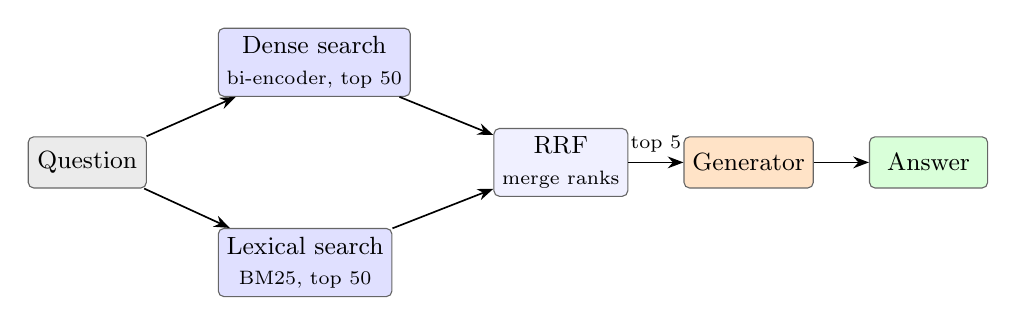
\begin{tikzpicture}[node distance=4mm and 7mm]
\node[q] (q) {Question};
\node[ret, above right=5mm and 9mm of q] (dense) {Dense search\\ \scriptsize bi-encoder, top 50};
\node[ret, below right=5mm and 9mm of q] (lex) {Lexical search\\ \scriptsize BM25, top 50};
\node[comp, fill=blue!6, right=44mm of q] (rrf) {RRF\\ \scriptsize merge ranks};
\node[llm, right=of rrf] (gen) {Generator};
\node[ans, right=of gen] (a) {Answer};
\draw[arr] (q) -- (dense); \draw[arr] (q) -- (lex);
\draw[arr] (dense) -- (rrf); \draw[arr] (lex) -- (rrf);
\draw[arr] (rrf) -- node[lbl, above] {top 5} (gen);
\draw[arr] (gen) -- (a);
\end{tikzpicture}
\caption{Hybrid retrieval. Dense and lexical rankings over the same corpus
are merged by Reciprocal Rank Fusion; the BM25 row is this diagram with
the dense branch removed.}
\label{fig:arch-hybrid}
\end{figure}

The two retrievers fail in different ways. The dense retriever understands
paraphrase but blurs rare surface forms (the lossy compression of
Supplementary Material, Section~S1); the lexical one matches names exactly but is
blind to a question that never uses the passage's vocabulary. Hybrid
retrieval runs both and merges the rankings with Reciprocal Rank
Fusion~\citep{cormack2009rrf}:
\begin{equation}
\mathrm{RRF}(d) \;=\; \sum_{r \,\in\, \text{rankings}} \frac{1}{k + r(d)},
\qquad k = 60,
\label{eq:rrf}
\end{equation}
where $r(d)$ is the rank of document $d$ in each list. RRF combines
\emph{ranks}, not scores, which is what makes the combination possible at
all: a cosine similarity and a BM25 score live on incomparable scales,
while their ranks do not. The BM25-only row is the same code with the dense
branch disabled, so the difference between the two rows measures exactly
``was the dense list fused in'' and nothing else. Cost: one extra lexical
search on the CPU; the generator is still called once.

\subsection{Rerank: cross-encoder reordering}
\label{sec:arch-rerank}

\begin{figure}[t]
\centering
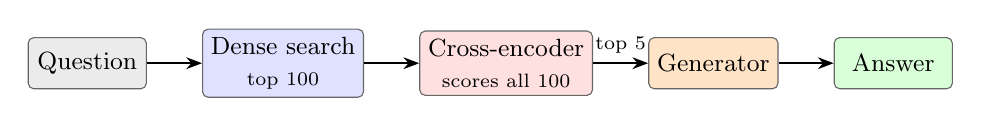
\begin{tikzpicture}[node distance=4mm and 7mm]
\node[q] (q) {Question};
\node[ret, right=of q] (dense) {Dense search\\ \scriptsize top 100};
\node[ret, right=of dense, fill=red!12] (ce) {Cross-encoder\\ \scriptsize scores all 100};
\node[llm, right=of ce] (gen) {Generator};
\node[ans, right=of gen] (a) {Answer};
\draw[arr] (q) -- (dense);
\draw[arr] (dense) -- (ce);
\draw[arr] (ce) -- node[lbl, above] {top 5} (gen);
\draw[arr] (gen) -- (a);
\end{tikzpicture}
\caption{Cross-encoder reranking: a deep bi-encoder shortlist is reordered
by a jointly-encoding relevance model; only the reordered top five reach
the generator.}
\label{fig:arch-rerank}
\end{figure}

A deep shortlist (100 candidates) is retrieved with the fast bi-encoder and
reordered with a cross-encoder (Supplementary Material, Section~S1); the top five
survivors reach the generator. The target failure is ``right article
ranked too low'': for a third of the diagnosed failures on 2WikiMultihopQA
the answer-bearing article is already in the ranking, just below the
cut-off, and nothing that reasons over the top five can recover it --- the
fix has to change which five are chosen. Unlike the iterative methods this
adds no generator call; the cost is one cross-encoder pass over the
shortlist.

\subsection{Neighbour expansion}
\label{sec:arch-neighbour}

Wikipedia articles are chunked into approx.\ 100-word passages with no regard
for where a fact ends, so the retriever can land on the paragraph about the
right entity while the sentence carrying the answer sits in the next chunk.
Neighbour expansion retrieves as NaiveRAG does, then adds, for every hit,
the passages adjacent to it in the same article (radius one, capped at
fifteen passages, $\sim$11.5 in practice). It is included in order to \emph{test}
the chunking hypothesis, not because our diagnosis supports it: the
``wrong slice'' bucket is only 5--14\% of failures. It is read against
the twelve-passage control, because its expanded context would
otherwise masquerade as a retrieval gain.

\subsection{HyDE: search with a hypothetical document}
\label{sec:arch-hyde}

\begin{figure}[t]
\centering
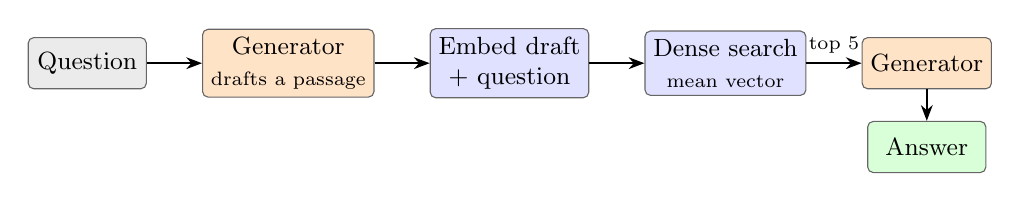
\begin{tikzpicture}[node distance=4mm and 7mm]
\node[q] (q) {Question};
\node[llm, right=of q] (draft) {Generator\\ \scriptsize drafts a passage};
\node[ret, right=of draft] (enc) {Embed draft\\ $+$ question};
\node[ret, right=of enc] (search) {Dense search\\ \scriptsize mean vector};
\node[llm, right=of search] (gen) {Generator};
\node[ans, below=of gen] (a) {Answer};
\draw[arr] (q) -- (draft);
\draw[arr] (draft) -- (enc);
\draw[arr] (enc) -- (search);
\draw[arr] (search) -- node[lbl, above] {top 5} (gen);
\draw[arr] (gen) -- (a);
\end{tikzpicture}
\caption{HyDE. The generator first writes the encyclopedia passage it
imagines would answer the question; the search runs on the average of the
draft's and the question's embeddings. The draft's factual errors are
discarded --- only its vector is used.}
\label{fig:arch-hyde}
\end{figure}

A question and a passage that answers it are different kinds of text:
``Where was the place of death of the director of film Beat Girl?'' shares
almost no vocabulary with a paragraph about Edmond T.\ Gr\'eville. HyDE
\citep{gao2022hyde} removes the mismatch by asking the generator to write
the passage it \emph{thinks} would answer the question and searching with
that instead. The draft is usually wrong in its details and it does not
matter: it only has to look like the right passage so that the encoder
places it near the real one. The question's own embedding is averaged in
as a safety net, so an off-topic draft degrades towards NaiveRAG instead
of chasing a hallucination. This targets the ``unreachable by this query''
failure bucket --- 53\% of failures on MuSiQue. Cost: one extra generator
call, the cheapest of the query-side methods.

\subsection{IRCoT: interleaved retrieval and reasoning}
\label{sec:arch-ircot}

\begin{figure}[t]
\centering
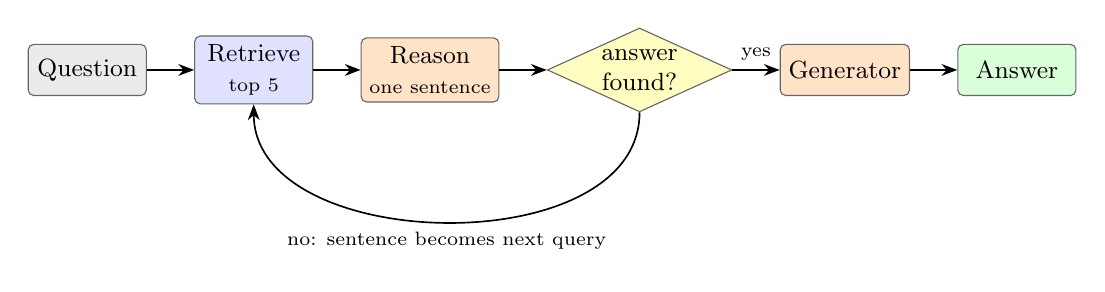
\begin{tikzpicture}[node distance=4mm and 6mm]
\node[q] (q) {Question};
\node[ret, right=of q] (r0) {Retrieve\\ \scriptsize top 5};
\node[llm, right=of r0] (step) {Reason\\ \scriptsize one sentence};
\node[dec, right=of step] (done) {answer\\found?};
\node[llm, right=of done] (gen) {Generator};
\node[ans, right=of gen] (a) {Answer};
\draw[arr] (q) -- (r0);
\draw[arr] (r0) -- (step);
\draw[arr] (step) -- (done);
\draw[arr] (done) -- node[lbl, above] {yes} (gen);
\draw[arr] (done.south) to[out=-90,in=-90] node[lbl, below] {no: sentence becomes next query} (r0.south);
\draw[arr] (gen) -- (a);
\end{tikzpicture}
\caption{IRCoT. Each reasoning sentence names entities the question never
mentioned, and is used verbatim as the next retrieval query; accumulated
passages (up to 15) go to the same reader prompt as NaiveRAG.}
\label{fig:arch-ircot}
\end{figure}

A single query built from the question alone is structurally insufficient
for multi-hop questions: ``What is the capital of the country where X was
born?'' never names the country, so no single query can reach the passage
that answers it. Measured on the baseline, recall over the context falls
from \NaiveRAGHotpotQARecallInContext{} on HotpotQA to
\NaiveRAGTwoWikiRecallInContext{} on 2WikiMultihopQA to
\NaiveRAGMuSiQueRecallInContext{} on MuSiQue as the number of required hops
grows. IRCoT~\citep{trivedi2023ircot} alternates: reason one sentence over
what has been retrieved, use that sentence as the next query, add what
comes back, repeat (up to four rounds or fifteen passages). The final
answer is produced by the same reader prompt as NaiveRAG over the
accumulated passages, so the only difference between the two systems is
the set of passages in context. We run a zero-shot variant and, because
the original method prompts the reasoning step with a worked example, a
one-shot variant with a single hand-written two-hop demonstration ---
identical for every question set --- as a separate row, so that a
under-prompted-baseline objection can be answered with data. Cost: two to
six generator calls per question.

\subsection{CRAG: corrective retrieval (offline, corpus-only)}
\label{sec:arch-crag}

\begin{figure}[t]
\centering
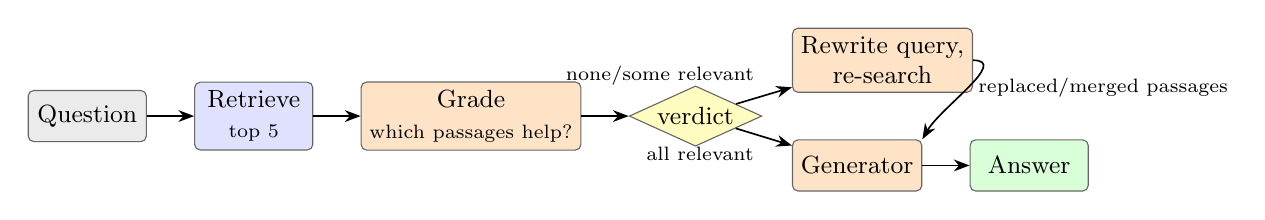
\begin{tikzpicture}[node distance=4mm and 6mm]
\node[q] (q) {Question};
\node[ret, right=of q] (r0) {Retrieve\\ \scriptsize top 5};
\node[llm, right=of r0] (grade) {Grade\\ \scriptsize which passages help?};
\node[dec, right=of grade] (branch) {verdict};
\node[llm, above right=1mm and 8mm of branch] (rewrite) {Rewrite query,\\re-search};
\node[llm, below right=1mm and 8mm of branch] (gen) {Generator};
\node[ans, right=of gen] (a) {Answer};
\draw[arr] (q) -- (r0);
\draw[arr] (r0) -- (grade);
\draw[arr] (grade) -- (branch);
\draw[arr] (branch) -- node[lbl, above left] {none/some relevant} (rewrite);
\draw[arr] (branch) -- node[lbl, below left] {all relevant} (gen);
\draw[arr] (rewrite.east) to[out=0,in=60] node[lbl, right] {replaced/merged passages} (gen.north east);
\draw[arr] (gen) -- (a);
\end{tikzpicture}
\caption{CRAG (offline form). The generator grades its own retrieval; on a
poor grade the query is rewritten and the corpus searched again, replacing
(no passage relevant) or topping up (some relevant) the context.}
\label{fig:arch-crag}
\end{figure}

NaiveRAG hands the generator whatever came back and hopes it is relevant;
the baseline measurements say how often that hope is misplaced (a gold
answer appears in the retrieved context for only
\NaiveRAGTwoWikiAnswerInContext{} of 2WikiMultihopQA questions).
CRAG~\citep{yan2024crag} adds the missing step: judge the retrieval before
using it, and act when it is bad. Our implementation deviates from the
paper in three deliberate, named ways, and is labelled ``CRAG (offline,
corpus-only)'' throughout: the generator itself grades relevance in one
call (the paper trains a T5 evaluator; a trained evaluator would confound
the controlled comparison with an extra model); the corrective action is a
query rewrite over the same corpus (the paper uses web search, which would
change the available knowledge, not the architecture); and the paper's
knowledge-refinement step is absent. A ten-passage variant pairs with the
matched-budget control. Cost: three generator calls per question.

\subsection{Adaptive-RAG: routing by predicted difficulty}
\label{sec:arch-adaptive}

\begin{figure}[t]
\centering
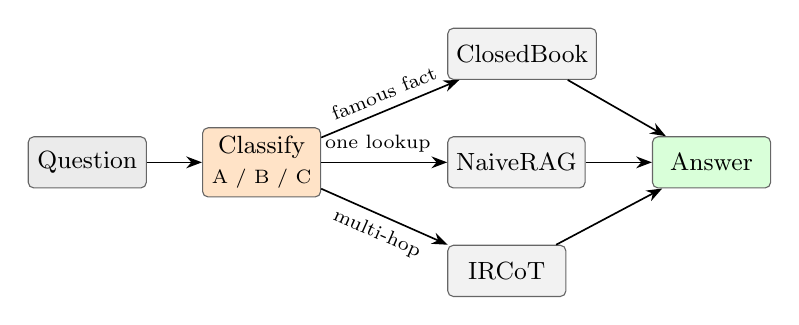
\begin{tikzpicture}[node distance=4mm and 7mm]
\node[q] (q) {Question};
\node[llm, right=of q] (route) {Classify\\ \scriptsize A / B / C};
\node[comp, fill=black!5, above right=6mm and 16mm of route] (cb) {ClosedBook};
\node[comp, fill=black!5, right=16mm of route] (naive) {NaiveRAG};
\node[comp, fill=black!5, below right=6mm and 16mm of route] (ircot) {IRCoT};
\node[ans, right=42mm of route] (a) {Answer};
\draw[arr] (q) -- (route);
\draw[arr] (route) -- node[lbl, above, sloped] {famous fact} (cb);
\draw[arr] (route) -- node[lbl, above, pos=0.45] {one lookup} (naive);
\draw[arr] (route) -- node[lbl, below, sloped] {multi-hop} (ircot);
\draw[arr] (cb) -- (a); \draw[arr] (naive) -- (a); \draw[arr] (ircot) -- (a);
\end{tikzpicture}
\caption{Adaptive-RAG (training-free form). One classification call routes
each question to the no-retrieval, single-step, or iterative branch; the
branches are the very architectures of the neighbouring rows.}
\label{fig:arch-adaptive}
\end{figure}

Every other architecture treats all questions alike, and the measurements
say that is wrong in both directions: on TriviaQA the generator already
knows \ClosedBookTriviaQAEM{} of the answers with no retrieval, so running
IRCoT over them spends up to six calls to arrive where one would have
done, while on MuSiQue a single query reaches the answer-bearing article
for barely a fifth of questions. Adaptive-RAG~\citep{jeong2024adaptiverag}
routes each question --- here with a single generator classification call
rather than the paper's trained classifier, for the same
no-extra-models reason as CRAG --- to closed-book, single-step, or IRCoT.
The router's branches are built from the same components as the
architectures they are compared against, so its row is comparable with
theirs by construction. Cost: one call plus whatever the chosen branch
costs (2.1--3.0 in practice).

\section{CascadeRAG: an abstention-triggered cascade}
\label{sec:cascade}

Three measured facts motivate the design. First, \emph{no single
architecture wins everywhere}: reranking is the strongest refinement on
HotpotQA and the worst failure on NaturalQuestions; HyDE leads on
NaturalQuestions and adds little elsewhere; the iterative methods pay two
to six calls on every question including the majority that a single call
answers just as well. Second, \emph{there is large headroom in choosing
per question}: an oracle that picked, per question, the better of
closed-book and the naive baseline would gain
\DiagTwoWikiOracleGain{} Exact Match on 2WikiMultihopQA over the better
single system --- an order of magnitude more than any single refinement
delivers. Third, \emph{the reader already signals which questions need
more work}: a 7B instruct model holding irrelevant passages does not
guess; it declines (``the provided documents do not contain\ldots'').
On 2WikiMultihopQA the naive baseline declines on
\NaiveRAGTwoWikiAbstentionRate{} of questions, against
\ClosedBookTwoWikiAbstentionRate{} for the closed-book reader that has
nothing to object to. A refusal after reading the evidence is a
\emph{posterior} judgement of exactly the quantity a router tries to
\emph{predict} from the question alone.

CascadeRAG turns that signal into control flow: answer cheaply, and only
when the reader itself says the evidence does not support an answer, try
differently. It has two components; in tables and figures the
architecture appears as ``Cascade''.

\subsection{Stage one: fused retrieval}
\label{sec:cascade-fused}

The natural first stage would be the strongest single-call architecture,
reranking --- but its collapse on NaturalQuestions makes it unsafe as a
default. The collapse has a mechanism, visible in the per-question dumps.
A cross-encoder matches what a question is \emph{asking for} while a
bi-encoder matches what it is \emph{asking about}: for ``where is the tv
show the curse of oak island filmed'' the cross-encoder promotes the three
shortlist passages that state a filming location --- for \emph{Stake
Land}, \emph{The Island}, and \emph{Come Outside} --- because each answers
``where was it filmed'' perfectly, and pushes out the passage naming the
right show, which says nothing about filming locations. Answer-in-context
falls from 0.727 to 0.510 and Exact Match with it
($-0.100$).

\begin{figure}[t]
\centering
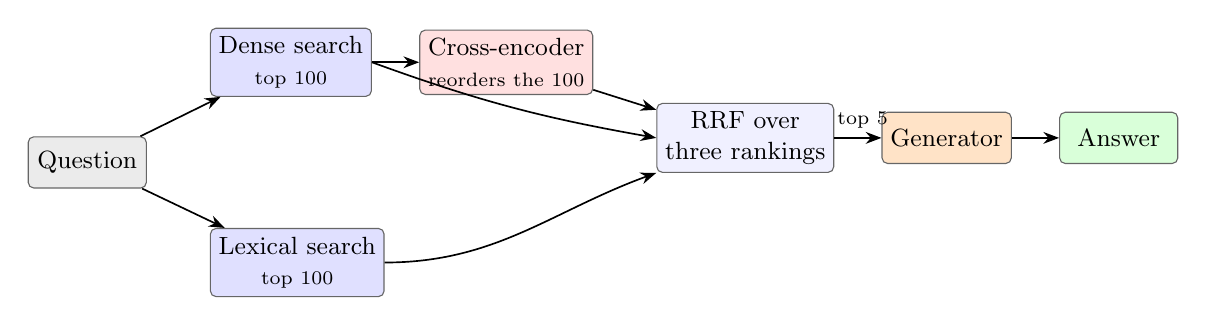
\begin{tikzpicture}[node distance=3.5mm and 6mm]
\node[q] (q) {Question};
\node[ret, above right=5mm and 8mm of q] (dense) {Dense search\\ \scriptsize top 100};
\node[ret, below right=5mm and 8mm of q] (lex) {Lexical search\\ \scriptsize top 100};
\node[ret, right=of dense, fill=red!12] (ce) {Cross-encoder\\ \scriptsize reorders the 100};
\node[comp, fill=blue!6, below right=1mm and 8mm of ce] (rrf) {RRF over\\ three rankings};
\node[llm, right=of rrf] (gen) {Generator};
\node[ans, right=of gen] (a) {Answer};
\draw[arr] (q) -- (dense); \draw[arr] (q) -- (lex);
\draw[arr] (dense) -- (ce);
\draw[arr] (dense.east) to[out=-20,in=170] (rrf.west);
\draw[arr] (ce) -- (rrf);
\draw[arr] (lex.east) to[out=0,in=-160] (rrf.south west);
\draw[arr] (rrf) -- node[lbl, above, pos=0.6] {top 5} (gen);
\draw[arr] (gen) -- (a);
\end{tikzpicture}
\caption{Fused retrieval, the cascade's first stage. The cross-encoder is
one voter among three rather than the arbiter: dense, lexical, and
reranked orderings of the same candidate pool are merged by RRF
(Eq.~\ref{eq:rrf}). A passage found by dense retrieval is voted for twice
(bi-encoder rank and cross-encoder rank); a passage only the lexical index
found is voted for once --- the lexical list is there to rescue passages
dense retrieval missed, not to outvote it.}
\label{fig:arch-fused}
\end{figure}

Fused retrieval (Figure~\ref{fig:arch-fused}) therefore demotes the
cross-encoder from arbiter to voter: the dense ranking, the cross-encoder's
reordering of it, and the lexical ranking are merged with the same RRF as
the hybrid baseline. Measured, the fusion is a compromise rather than a
free lunch --- on NaturalQuestions it scores 0.325 where rerank collapses
to \RerankNQEM{} (naive: \NaiveRAGNQEM); on HotpotQA it scores 0.351
against rerank's \RerankHotpotQAEM{} --- it avoids the catastrophe and
gives back part of the gain. Its case is robustness: of the candidate
first stages we measure, it has the best mean over the five sets and the
smallest worst-case loss (Section~\ref{sec:results-ablations}). Cost over
plain reranking: one lexical search on the CPU; the generator is still
called once.

\subsection{Stage two and three: escalation on abstention}
\label{sec:cascade-escalation}

\begin{figure}[t]
\centering
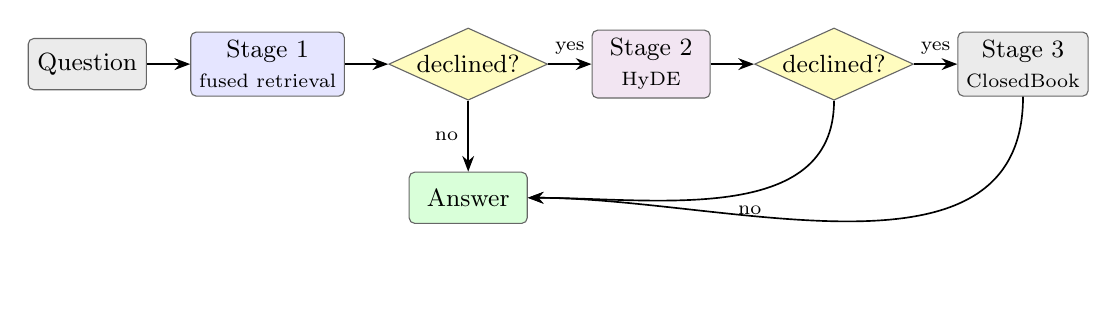
\begin{tikzpicture}[node distance=3.5mm and 5.5mm]
\node[q] (q) {Question};
\node[comp, fill=blue!10, right=of q] (s1) {Stage 1\\ \scriptsize fused retrieval};
\node[dec, right=of s1] (d1) {declined?};
\node[comp, fill=violet!10, right=of d1] (s2) {Stage 2\\ \scriptsize HyDE};
\node[dec, right=of s2] (d2) {declined?};
\node[comp, fill=black!8, right=of d2] (s3) {Stage 3\\ \scriptsize ClosedBook};
\node[ans, below=9mm of d1] (a1) {Answer};
\draw[arr] (q) -- (s1);
\draw[arr] (s1) -- (d1);
\draw[arr] (d1) -- node[lbl, above] {yes} (s2);
\draw[arr] (s2) -- (d2);
\draw[arr] (d2) -- node[lbl, above] {yes} (s3);
\draw[arr] (d1) -- node[lbl, left] {no} (a1);
\draw[arr] (d2.south) to[out=-90,in=0] node[lbl, below right] {no} (a1.east);
\draw[arr] (s3.south) to[out=-90,in=0] (a1.east);
\end{tikzpicture}
\caption{The cascade. A stage's answer is kept unless the reader declined;
only declined questions pay for the next stage. The last stage's answer is
kept whatever it says --- a refusal is still the most honest answer
available.}
\label{fig:arch-cascade}
\end{figure}

Declined questions are handed to HyDE --- whose drafted-passage search
reaches articles the fused query could not, the dominant remaining failure
--- and, if HyDE's reader declines too, to closed-book, which at least
recovers the guessing behaviour that abstention suppressed. Abstention is
detected heuristically: an explicit refusal phrase, or an answer longer
than twenty words where the gold answers are short spans; the threshold is
a stated hyperparameter.

Two properties distinguish this trigger from prior adaptive systems.

\paragraph{It is posterior.} Adaptive-RAG asks the generator to predict,
from the question alone, how much work the question will need --- and
gains $+0.0004$ Exact Match on 2WikiMultihopQA for it, routing 92\% of
that multi-hop set down the single-hop branch. The cascade's signal fires
\emph{after} the evidence has been seen: it is not a prediction of whether
retrieval will fail but a report that it did.

\paragraph{It is lossless under Exact Match.} An abstention is a sentence;
the gold answers in these datasets are short spans; a sentence cannot
normalise to a short span, so an abstention cannot score Exact Match~1 ---
verified exhaustively over all 887{,}917 (question, architecture) pairs
measured in this study, with zero exceptions. Escalating a declined
question therefore \emph{cannot discard a correct answer}: it can only
move a question from certainly-wrong to possibly-right. In the vocabulary
of selective prediction~\cite{chow1970reject,geifman2017selective}, the
refusal is a reject option whose selective risk is provably zero under
this metric. This is what makes the cascade safe by construction where
confidence-threshold deferral is a gamble; it is exact for Exact Match and approximate for token-level F1,
where an abstention averages 0.05 and exceeds 0.5 for 0.09\% of questions.

The ordering of stages follows their measured cost and coverage: fused
answers every question it can at one call; HyDE is the cheapest method
that reaches differently (two calls, only for the escalated minority);
closed-book costs one call and cannot itself retrieve badly. Only declined
questions pay for later stages, which is why the whole cascade averages
1.16--1.58 generator calls per question while containing a two-call and a
one-call stage.

\subsection{A second, continuous trigger: answer confidence}
\label{sec:cascade-confidence}

The abstention trigger is blind to the failure it cannot see: a wrong
answer given \emph{without} hesitation. The one free signal about those is
the generator's own certainty --- a signal language models are reported
to carry~\cite{kadavath2022know}, though eliciting it reliably is
hard~\cite{xiong2024uncertainty} --- here the mean log-probability of the
answer's tokens under greedy decoding, which the serving engine reports
at no extra cost. As an extension, the cascade also escalates any answer whose mean
token log-probability falls below a threshold $\tau$. Unlike the
abstention this is \emph{not} lossless --- a correct answer given with low
confidence is discarded and only sometimes recovered --- so $\tau$ is a
true hyperparameter, and we select it on 1{,}000 sampled questions from
each \emph{training} split, never on the test sets, by composing
independently-run stages question by question offline (exact under greedy
decoding, since every stage is deterministic given the question). Whether
this second trigger pays at all is an empirical question, answered ---
negatively --- in Section~\ref{sec:results-ablations}.

\subsection{Reading the cascade's numbers fairly}
\label{sec:cascade-caveats}

Three caveats belong in any honest report of this architecture, and we
state them before the results. Questions that reach the closed-book stage
end with no passages in context, so the cascade's aggregate retrieval
metrics are averages over a mixture and are not comparable with a pure
retrieval system's; it must be compared on answer quality. Its abstention
rate is the \emph{last} stage's, so ``Exact Match over questions both
systems answered'' compares different populations when set against a
single-stage system. And the gain, by design, sits in the questions the
first stage declined --- against reranking, Exact Match restricted to
questions both answered is at or below zero on four of five sets. The
cascade does not answer better where its first stage already answered; it
rescues the questions where the first stage knew it had failed. That is
what the design predicts, and the tables of
Section~\ref{sec:results} should be read with it in mind.

\section{Experimental setup}
\label{sec:setup}

\subsection{Unified settings}
\label{sec:setup-unified}

Every architecture runs against the same stack; the only variable between
two rows of any table is the architecture itself.

\begin{itemize}
\item \textbf{Corpus:} the FlashRAG release of \texttt{wiki18\_100w}
  \citep{jin2024flashrag} --- the December 2018 English Wikipedia snapshot
  chunked into 21{,}015{,}324 passages of $\sim$100 words, the first line
  of each passage being its article title.
\item \textbf{Dense index:} \texttt{bge-base-en-v1.5}~\citep{xiao2023bge}
  embeddings (768 dimensions, cosine similarity) in Qdrant, HNSW with a
  fixed search width (\texttt{ef}~$=256$; raised to 1024 where a deeper
  shortlist is requested, so the graph walk never limits a ranking the
  architecture needs). For this encoder the documented convention is no
  instruction prefix on either side; we verified over 500 held-out
  questions that adding the legacy BGE query instruction changes no
  retrieval metric beyond its bootstrap interval.
\item \textbf{Lexical index:} the same corpus and passage ids under BM25
  ($k_1{=}1.2$, $b{=}0.75$) in a separate sparse collection, so the two
  retrievers can be fused by passage id.
\item \textbf{Cross-encoder:} \texttt{bge-reranker-base} over the dense
  top-100.
\item \textbf{Generator:} Qwen2.5-7B-Instruct~\citep{qwen2025qwen25} served
  by vLLM~\citep{kwon2023vllm}, greedy decoding (temperature 0, so every
  run is reproducible), 64-token cap on answers, 256 on intermediate
  generations (a reasoning sentence truncated at the answer's cap would be
  half a sentence, then used verbatim as a retrieval query). All
  architectures share one answer prompt (``Answer the question based on
  the given documents. Only give me the answer\ldots'';
  Supplementary Material, Section~S3), so a score difference measures the passages
  in context, not answer formatting. The second-reader replication
  (Section~\ref{sec:results-reader}) swaps in
  Llama-3.1-8B-Instruct~\citep{grattafiori2024llama3} and changes nothing
  else.
\end{itemize}

\subsection{Question sets}
\label{sec:setup-datasets}

\begin{table}[t]
\centering\small
\caption{Question sets (FlashRAG splits). Recall ceiling is the mean
fraction of a question's gold articles present in the corpus at all
(Section~\ref{sec:setup-metrics}); NaturalQuestions and TriviaQA annotate
no gold documents.}
\label{tab:datasets}
\begin{tabular}{lrlrr}
\toprule
Question set & Questions & Type & Gold docs & Recall ceiling \\
\midrule
NaturalQuestions~\citep{kwiatkowski2019nq} & \NaiveRAGNQQuestions{} & single-hop & no & --- \\
TriviaQA~\citep{joshi2017triviaqa} & \NaiveRAGTriviaQAQuestions{} & single-hop & no & --- \\
HotpotQA~\citep{yang2018hotpotqa} & \NaiveRAGHotpotQAQuestions{} & 2-hop & yes & \CoverageHotpotQARecallCeiling{} \\
2WikiMultihopQA~\citep{ho20202wiki} & \NaiveRAGTwoWikiQuestions{} & 2--4-hop & yes & \CoverageTwoWikiRecallCeiling{} \\
MuSiQue~\citep{trivedi2022musique} & \NaiveRAGMuSiQueQuestions{} & 2--4-hop & yes & \CoverageMuSiQueRecallCeiling{} \\
\bottomrule
\end{tabular}
\end{table}

Table~\ref{tab:datasets} lists the five sets: two single-hop open-domain
sets and three multi-hop sets of increasing compositional depth.
Evaluation always runs on the dev or test split; the train splits are used
only to tune the cascade's confidence threshold
(Section~\ref{sec:cascade-confidence}) and never touch any reported table.

\subsection{Metrics}
\label{sec:setup-metrics}

\paragraph{Answer quality.} \emph{Exact Match} (EM): the normalised answer
(lower-cased, punctuation and articles stripped --- the standard SQuAD
normalisation~\citep{rajpurkar2016squad}) equals one of the gold answers;
the primary endpoint throughout. \emph{Token-level F1} against the best-matching gold answer.
The reader is instructed to output only the answer because the gold
answers are short spans; without that instruction an instruct model's
correct-but-verbose replies score EM~0 (measured: constraining the output
moves EM from 0.02 to 0.40 on a HotpotQA subsample without touching
retrieval).

\paragraph{Abstention.} EM cannot tell a refusal from a wrong guess, and
the two say opposite things about a system. An answer is counted as an
abstention on an explicit refusal phrase or when longer than twenty words.
We report the abstention rate and EM restricted to answered
questions; Section~\ref{sec:results-worth} shows a ranking that reverses
without them.

\paragraph{Retrieval quality.} \emph{Recall in context}: the fraction of a
question's gold articles among the passages actually placed in the
generator's context --- deliberately not ``Recall@$k$'', because iterative
architectures accumulate more than $k$ passages, so the mean context size
is reported beside it and the budget-matched controls make comparisons
fair. Article titles are compared after Unicode normalisation; the corpus
and the question sets disagree on the encoding of accented characters
often enough that a byte comparison silently loses 4.5\% of
2WikiMultihopQA's gold articles. \emph{MRR}; and \emph{answer-in-context}
--- whether a gold answer appears as a run of whole tokens in a retrieved
passage --- for the two sets without gold-document annotation (matching
whole tokens, because a substring test scores 0.97 for questions whose
gold answer is ``no'', which occurs inside ``north'' and ``known'').

\paragraph{The corpus ceiling.} A recall figure is unreadable without the
ceiling the corpus imposes: only \CoverageTwoWikiRecallCeiling{} of
2WikiMultihopQA's gold articles exist in \texttt{wiki18\_100w} at all, so
a perfect retriever would score \CoverageTwoWikiRecallCeiling{} there, and
the baseline's \NaiveRAGTwoWikiRecallInContext{} is about half of what is
achievable, not a third of it. We measure the ceiling per question set
(Table~\ref{tab:datasets}) and read every recall against it.

\paragraph{Cost.} Generator calls and prompt/completion tokens per
question, read from the per-question logs --- the only cost measure
comparable across hardware. Latency is reported nowhere: at the
concurrency the runs used, per-question timing measures the queue, and
runs at identical token counts differ in wall-clock by a factor of two
depending on what else shared the GPU. The cross-encoder pass and the CPU
lexical search are outside the token count and are stated as such
where they apply.

\subsection{Statistical protocol}
\label{sec:setup-stats}

Both systems of every comparison answered the same questions, so all tests
are paired, which removes question difficulty from the variance ---
two overlapping confidence intervals can hide a consistent per-question
win. Exact Match and the other binary metrics use McNemar's
test~\citep{mcnemar1947} on the discordant pairs; continuous metrics use
the Wilcoxon signed-rank test~\citep{wilcoxon1945}; the size of every
difference carries a paired bootstrap~\citep{efron1979bootstrap} 95\%
interval (10{,}000 resamples, fixed seed). Because a dozen metrics are
tested per comparison, p-values are Holm-adjusted~\citep{holm1979} within
each comparison, with Exact Match the pre-declared primary endpoint. The
headline table (Table~\ref{tab:main}) is stricter still: its claim ---
``wins $W$, loses $L$, ties $T$ of $P$ pairs'' --- is one family of tests,
so Holm runs over every cell of the table at once, and several narrow
per-pair wins are ties there.

\subsection{Reproducibility}
\label{sec:setup-repro}

Every run writes one JSON line per question --- answer, scores, retrieved
passage ids and titles, token counts, and the architecture's internal
decisions (which CRAG branch fired, which cascade stage answered, every
IRCoT reasoning sentence). All aggregate tables, all significance tests,
and all numbers in this manuscript are generated from those logs by the
benchmark tools and imported as named macros; no number is typed by hand.
One make target per experiment reproduces the corresponding rows
end-to-end. The complete pipeline --- benchmark code, analysis tools,
per-question logs, generated fragments, and the source of this manuscript
--- is available at \url{https://github.com/mikolajsemeniuk/ragbench}.

\section{Results}
\label{sec:results}

We organise the results as six questions. Full per-set tables for every
architecture and metric are in Supplementary Material, Section~S2; unless
stated otherwise, differences quoted below are paired Exact Match
differences with Holm-adjusted p-values, and ``significant'' means
$p<0.05$ after adjustment.

\subsection{RQ1: is retrieval worth anything at all?}
\label{sec:results-worth}

Against the closed-book bottom line, naive retrieval is worth
\ClosedBookVsNaiveNQExactMatchDiff{} EM on NaturalQuestions,
\ClosedBookVsNaiveTriviaQAExactMatchDiff{} on TriviaQA,
\ClosedBookVsNaiveHotpotQAExactMatchDiff{} on HotpotQA, and
\ClosedBookVsNaiveMuSiQueExactMatchDiff{} on MuSiQue --- large,
significant gains everywhere except one set. On 2WikiMultihopQA the naive
row appears to \emph{lose} to no retrieval at all
(\ClosedBookVsNaiveTwoWikiExactMatchDiff{} EM), and this apparent
inversion is an abstention artefact, not a knowledge difference: holding
irrelevant passages, the reader declines on
\NaiveRAGTwoWikiAbstentionRate{} of questions (closed-book:
\ClosedBookTwoWikiAbstentionRate), and a decline scores zero where a
closed-book \emph{guess} is sometimes right. Restricted to questions both
systems answered, the ordering reverses
(\ClosedBookVsNaiveTwoWikiEMbothansweredDiff{} in naive's favour). Any
evaluation that reports EM without abstention would publish the wrong
conclusion on this set --- which is why every table in this article
carries both.

\subsection{RQ2: what does each single refinement buy?}
\label{sec:results-single}

\paragraph{Lexical and hybrid retrieval.} BM25 alone is well below the
dense baseline on the open-domain sets
(\NaiveVsBMTwentyFiveNQExactMatchDiff{} on NaturalQuestions) but
\emph{ahead} of it on 2WikiMultihopQA
(\NaiveVsBMTwentyFiveTwoWikiExactMatchDiff), whose questions name their
target articles verbatim --- exactly the rare-surface-form failure of
Supplementary Material, Section~S1. Fusing the two (Hybrid) is a small but
uniformly non-negative improvement
(\NaiveVsHybridNQExactMatchDiff{} to
\NaiveVsHybridTwoWikiExactMatchDiff{} across sets) at one CPU search of
extra cost --- the cheapest strictly-safe refinement measured here.

\paragraph{Cross-encoder reranking.} The strongest single gain and the
worst single failure, on different sets: \NaiveVsRerankHotpotQAExactMatchDiff{}
on HotpotQA and \NaiveVsRerankTwoWikiExactMatchDiff{} on 2WikiMultihopQA,
against \NaiveVsRerankNQExactMatchDiff{} on NaturalQuestions, where
answer-in-context falls from \NaiveRAGNQAnswerInContext{} to
\RerankNQAnswerInContext{} by the asking-for/asking-about mechanism of
Section~\ref{sec:cascade-fused}. Reranking is a bet on the question
distribution, not a safe default.

\paragraph{HyDE.} The one refinement that beats the baseline on
NaturalQuestions (\NaiveVsHyDENQExactMatchDiff{}, answer-in-context
\NaiveRAGNQAnswerInContext{} $\rightarrow$ \HyDENQAnswerInContext) and it
helps on the multi-hop sets as well
(\NaiveVsHyDETwoWikiExactMatchDiff{} on 2WikiMultihopQA), at the fixed
price of doubling the generator calls on every question.

\paragraph{Neighbour expansion.} Read against the twelve-passage control,
expansion is worth \NaiveTwelveVsNeighbourHotpotQAExactMatchDiff{} on
HotpotQA, \NaiveTwelveVsNeighbourTwoWikiExactMatchDiff{} on
2WikiMultihopQA and \NaiveTwelveVsNeighbourMuSiQueExactMatchDiff{} on
MuSiQue --- a null result, and a predicted one: the diagnosis
(RQ3) puts the ``wrong slice of the right article'' bucket this method
repairs at 5--14\% of failures. The popular advice to always fetch
neighbouring chunks is, on this corpus, worth approximately nothing once
context size is controlled.

\paragraph{Iterative and corrective methods.} Against the matched
ten-passage control, IRCoT gains
\NaiveTenVsIRCoTHotpotQAExactMatchDiff{} on HotpotQA,
\NaiveTenVsIRCoTTwoWikiExactMatchDiff{} on 2WikiMultihopQA and
\NaiveTenVsIRCoTMuSiQueExactMatchDiff{} on MuSiQue at 2.1--2.5 calls per
question; the one-shot variant with a worked example changes little
(\IRCoTVsIRCoTOneShotHotpotQAExactMatchDiff{} on HotpotQA,
\IRCoTVsIRCoTOneShotTwoWikiExactMatchDiff{} on 2WikiMultihopQA), because
the zero-shot loop already declares itself able to answer after the first
round --- the same five passages NaiveRAG reads --- on 70--80\% of
multi-hop questions. CRAG at the same budget gains
\NaiveTenVsCRAGTenMuSiQueExactMatchDiff{} on MuSiQue, its best set, at
three calls per question. Adaptive routing is indistinguishable from its
own single-hop branch (\NaiveVsAdaptiveTwoWikiExactMatchDiff{} vs.\ naive
on 2WikiMultihopQA): predicting difficulty from the question alone sends
92\% of a multi-hop set down the single-hop path.

\subsection{RQ3: why does retrieval fail?}
\label{sec:results-diagnosis}

\begin{table}[t]
\centering\small
\caption{Diagnosis of the naive baseline's retrieval failures (300 sampled
failures per set; percentages of the diagnosed sample). The last row is
the Exact Match an oracle choosing per question between the naive run and
closed-book would add over the better single system.}
\label{tab:diagnosis}
\begin{tabular}{lrrr}
\toprule
Failure cause & HotpotQA & 2Wiki & MuSiQue \\
\midrule
Wrong slice of the right article & \DiagHotpotQAWrongSlicePct\% & \DiagTwoWikiWrongSlicePct\% & \DiagMuSiQueWrongSlicePct\% \\
Right article ranked 11--1000 & \DiagHotpotQARankedLowPct\% & \DiagTwoWikiRankedLowPct\% & \DiagMuSiQueRankedLowPct\% \\
Unreachable by this query & \DiagHotpotQAUnreachablePct\% & \DiagTwoWikiUnreachablePct\% & \DiagMuSiQueUnreachablePct\% \\
No gold article states the answer & \DiagHotpotQAAnswerAbsentPct\% & \DiagTwoWikiAnswerAbsentPct\% & \DiagMuSiQueAnswerAbsentPct\% \\
Gold article not in the corpus & \DiagHotpotQANotInCorpusPct\% & \DiagTwoWikiNotInCorpusPct\% & \DiagMuSiQueNotInCorpusPct\% \\
\midrule
Oracle (retrieve-or-closed-book) gain & \DiagHotpotQAOracleGain{} & \DiagTwoWikiOracleGain{} & \DiagMuSiQueOracleGain{} \\
\bottomrule
\end{tabular}
\end{table}

Table~\ref{tab:diagnosis} splits the baseline's failures into the five
causes of Section~\ref{sec:naive-pipeline}, each demanding a different
remedy. Three readings matter. First, the two \emph{unfixable} buckets ---
answer not stated by any gold article, article absent from the corpus ---
account for roughly a quarter to a third of failures, which is the
concrete form of the recall ceiling. Second, the \emph{ranking} bucket
(article present, reachable, ranked 11--1000) is the largest fixable one
on HotpotQA and 2WikiMultihopQA --- which is why reranking is the
strongest single refinement there --- while on MuSiQue the
\emph{unreachable} bucket dominates at \DiagMuSiQueUnreachablePct\%,
which is why query-side methods are what helps there. Third, the
\emph{wrong slice} bucket that neighbour expansion repairs is small
everywhere, predicting that method's null result. The diagnosis, made
before the cascade was designed, is the design brief the cascade answers:
fuse rankings (largest bucket), escalate to a query-side method
(second bucket), fall back to no retrieval (the questions where
retrieval cannot help but a guess might).

\subsection{RQ4: the cascade against every baseline}
\label{sec:results-main}

\begin{table}[t]
\centering\small
\caption{The proposed cascade against every baseline on every question
set. Each cell is the paired Exact Match difference (cascade minus
baseline); \textbf{bold} marks a significant cascade win and
\underline{underline} a significant loss under McNemar's test with Holm
adjustment over all \ResultPairs{} cells jointly. The cascade wins
\ResultWins{}, loses \ResultLosses{}, ties \ResultTies{}.}
\label{tab:main}
\ResultTable
\end{table}

Table~\ref{tab:main} is the headline result: \ResultWins{} significant
wins, \ResultLosses{} loss, \ResultTies{} ties over \ResultPairs{}
(baseline, question set) pairs, under the strictest correction. Against
the standard baseline the cascade gains
\NaiveVsCascadeTriviaQAExactMatchDiff{} on TriviaQA,
\NaiveVsCascadeHotpotQAExactMatchDiff{} on HotpotQA,
\NaiveVsCascadeTwoWikiExactMatchDiff{} on 2WikiMultihopQA and
\NaiveVsCascadeMuSiQueExactMatchDiff{} on MuSiQue; on NaturalQuestions the
difference (\NaiveVsCascadeNQExactMatchDiff) is not significant --- the
one set where the baseline was already near its measured ceiling for this
reader. The single loss is to reranking on HotpotQA
(\RerankVsCascadeHotpotQAExactMatchDiff), the set where the
cross-encoder's bet pays; against the same reranking on NaturalQuestions
the cascade gains \RerankVsCascadeNQExactMatchDiff. No other architecture
in the study has a row without a significant loss; several
(rerank, HyDE, CRAG-10) beat the cascade on their single best set. The
cascade's claim is not ``best everywhere'' but \emph{never worse than the
baseline, never catastrophic, at near-baseline cost} --- and
Table~\ref{tab:main} is that claim in test form.

Where does the gain come from? The stage distribution says: the fused
first stage answers \CascadeNQStageFused{} of \CascadeNQQuestions{}
NaturalQuestions questions, \CascadeTriviaQAStageFused{} of
\CascadeTriviaQAQuestions{} on TriviaQA, and
\CascadeMuSiQueStageFused{} of \CascadeMuSiQueQuestions{} on MuSiQue ---
the escalated remainder splits between HyDE
(e.g.\ \CascadeMuSiQueStageHyde{} on MuSiQue) and closed-book
(\CascadeMuSiQueStageClosedbook). The cascade's own abstention rate
collapses to \CascadeTriviaQAAbstentionRate--\CascadeMuSiQueAbstentionRate{}
(baseline: \NaiveRAGTriviaQAAbstentionRate--\NaiveRAGMuSiQueAbstentionRate),
because a question must be declined by \emph{three} strategies to end in a
refusal. Consistent with Section~\ref{sec:cascade-caveats}, EM restricted
to questions both systems answered is at or below zero against reranking
on four of five sets: the cascade wins by rescuing declined questions,
not by answering differently where its first stage already answered.

\subsection{RQ5: what does it cost?}
\label{sec:results-cost}

\begin{table}[t]
\centering\small
\caption{Cost per question, averaged over the sets each architecture ran
on, from the per-question logs. The last column is prompt tokens relative
to the naive baseline. The cross-encoder pass (rerank, fused, cascade) and
the CPU lexical search (BM25, hybrid, fused, cascade) are outside the
token count.}
\label{tab:cost}
\resizebox{\textwidth}{!}{\CostTable}
\end{table}

Table~\ref{tab:cost} prices every row. The cascade averages
\CostcascadeCalls{} generator calls and \CostcascadePromptRatio$\times$ the
baseline's prompt tokens --- against $2$--$3\times$ calls and
$2.2$--$4\times$ tokens for the corrective and iterative methods it
outperforms in Table~\ref{tab:main}. Figure~\ref{fig:pareto} plots both
dimensions: the cascade and its own first stage bound the quality--cost
frontier at each end, and every architecture that spends more than 1.6
calls per question sits strictly inside it. Escalation prices the
expensive strategies by the questions that need them: HyDE costs two
calls \emph{per escalated question}, and only 10--30\% of questions
escalate.

\subsection{RQ6: which parts of the cascade matter?}
\label{sec:results-ablations}

\paragraph{What the fusion adds.} Stage one alone against plain reranking:
\RerankVsFusedNQExactMatchDiff{} on NaturalQuestions and
\RerankVsFusedHotpotQAExactMatchDiff{} on HotpotQA --- the fusion buys
back the collapse at the price of part of the gain, and its mean over the
five sets (0.322) is the best of any single-call architecture measured.
Swapping the first stage confirms the choice: a rerank-first cascade beats
the fused-first one on HotpotQA
(\CascadeRerankVsCascadeHotpotQAExactMatchDiff{} for fused-first) but
loses \CascadeRerankVsCascadeNQExactMatchDiff{} on NaturalQuestions; a
naive-first cascade is close behind everywhere
(\CascadeNaiveVsCascadeTwoWikiExactMatchDiff{} on 2WikiMultihopQA) and is
the cheapest variant; hybrid-first sits between
(\CascadeHybridVsCascadeNQExactMatchDiff{} on NaturalQuestions). No first
stage wins everywhere; fused has the best mean and the smallest
worst-case loss, which is its case.

\paragraph{What the escalation adds.} The cascade against its own first
stage run without escalation: \FusedVsCascadeNQExactMatchDiff{} on
NaturalQuestions, \FusedVsCascadeTriviaQAExactMatchDiff{} on TriviaQA,
\FusedVsCascadeHotpotQAExactMatchDiff{} on HotpotQA,
\FusedVsCascadeTwoWikiExactMatchDiff{} on 2WikiMultihopQA,
\FusedVsCascadeMuSiQueExactMatchDiff{} on MuSiQue --- one to three points
on every set, all significant, for 0.16--0.58 extra calls. The escalation
is worth roughly this much on top of \emph{any} first stage we tried;
which first stage is best depends on the set, but that the escalation
helps does not.

\paragraph{The confidence trigger does not pay.} The sweep over
\SweepQuestions{} held-out train questions puts the best threshold at
\SweepBestThreshold{} for a gain of $+0.0018$ EM over the abstention-only
cascade ($p=0.42$) at $+0.25$ calls per question. At that threshold on the
test sets, the trigger fires on 9--15\% of questions and the paired
difference against the abstention-only cascade is
\CascadeVsCascadeLogprobNQExactMatchDiff{} on NaturalQuestions,
\CascadeVsCascadeLogprobTriviaQAExactMatchDiff{} on TriviaQA,
\CascadeVsCascadeLogprobHotpotQAExactMatchDiff{} on HotpotQA,
\CascadeVsCascadeLogprobTwoWikiExactMatchDiff{} on 2WikiMultihopQA (the
one significant difference --- a loss) and
\CascadeVsCascadeLogprobMuSiQueExactMatchDiff{} on MuSiQue, at 0.2--0.36
extra calls. The greedy reader is nearly as confident when wrong as when
right: its token log-probabilities carry almost no information the
abstention did not already carry. We report this negative result because
the opposite is widely assumed; the abstention-only cascade remains the
proposed configuration. (Full sweep in Supplementary Material, Section~S3.)

\paragraph{The one-shot IRCoT objection.} Prompted with a worked example
as the original method prescribes, IRCoT changes by
\IRCoTVsIRCoTOneShotHotpotQAExactMatchDiff{} on HotpotQA and
\IRCoTVsIRCoTOneShotTwoWikiExactMatchDiff{} on 2WikiMultihopQA relative
to the zero-shot loop, and the cascade's comparison against it
(\IRCoTOneShotVsCascadeTwoWikiExactMatchDiff{} on 2WikiMultihopQA at
$2.4$ vs.\ $1.3$ calls) is materially the same as against the zero-shot
row. The multi-hop baseline was not under-prompted.

\subsection{RQ7: does it survive a different reader?}
\label{sec:results-reader}

Everything the cascade claims rests on how a reader behaves when the
passages are irrelevant --- it must decline rather than guess. One model
is not evidence that readers in general do that, so the rows the claims
stand on (closed-book, naive, rerank, fused, cascade) were re-run with
Llama-3.1-8B-Instruct over the same index and questions, changing nothing
else. The pattern transfers: the cascade wins \ResultLlamaWins{} of
\ResultLlamaPairs{} pairs, loses \ResultLlamaLosses{}, ties
\ResultLlamaTies{} (Holm over the table), with the same signature ---
large gains over reranking on NaturalQuestions
(\RerankVsCascadeLlamaNQExactMatchDiff), a small loss to it on HotpotQA
(\RerankVsCascadeLlamaHotpotQAExactMatchDiff), significant gains over the
naive baseline on every set, and the escalation worth
\FusedVsCascadeLlamaNQExactMatchDiff{} to
\FusedVsCascadeLlamaTwoWikiExactMatchDiff{} over stage one alone. The
full second-reader table is in Supplementary Material, Section~S2.

\section{Discussion: lessons for practitioners and evaluators}
\label{sec:discussion}

The benchmark supports several pieces of guidance that are more general
than any single row of the tables.

\paragraph{No retrieval refinement is universally safe --- except the
boring one.} Every advanced method measured here loses to the naive
baseline on at least one question set, with one exception: hybrid
dense-plus-BM25 fusion, which is small, positive everywhere, and nearly
free. A practitioner who can afford exactly one change should make that
one. The refinements with headline gains (reranking, HyDE, iterative
retrieval) are bets on a question distribution and should be preceded by
the diagnosis of Section~\ref{sec:results-diagnosis} on a sample of the
actual workload --- the failure-cause split, not the aggregate recall,
predicts which bet pays.

\paragraph{Compare at matched budget, or measure context size by
accident.} Ten passages instead of five is worth $+0.02$ EM on a multi-hop
set before any architectural idea enters. Neighbour expansion looks like a
retrieval improvement against the five-passage baseline and dissolves
against the twelve-passage control. Any comparison whose systems place
different amounts of text in the context is confounded until proven
otherwise.

\paragraph{Report abstention, or Exact Match will lie.} A reader holding
irrelevant evidence declines; a reader holding nothing guesses; EM scores
the decline zero and the lucky guess one. That artefact alone reverses the
closed-book-versus-RAG ordering on 2WikiMultihopQA. Abstention rate and
EM-over-answered belong next to EM in every RAG table.

\paragraph{Posterior signals beat prior predictions.} Asking a model
whether a question \emph{will} need retrieval (routing) bought $+0.0004$
EM; acting on the reader's report that retrieval \emph{did} fail bought
one to three points on every set at a fraction of the cost of always
escalating. The reader's refusal is the cheapest reliable difficulty
signal in the system, and it is already being generated --- most
pipelines simply throw it away.

\paragraph{Confidence is not a second signal --- at least not for free.}
The mean token log-probability of a greedily decoded answer, the most
commonly proposed deferral signal, carried no information beyond the
abstention it accompanies: tuned on held-out data, it bought $+0.0018$ EM
at $+0.25$ calls and lost significantly on one test set. Calibration
should be measured before a confidence threshold is trusted.

\paragraph{Report the ceiling.} Only \CoverageTwoWikiRecallCeiling{} of
2WikiMultihopQA's gold articles exist in the standard corpus; a quarter
of ``retrieval failures'' there are unfixable by any retriever. Recall
reported without the corpus ceiling overstates the room architectures
have to differ --- and, we suspect, explains part of the literature's
replication noise on this set.

\paragraph{Escalation prices expensive methods correctly.} The cascade is
not a new retrieval method; it is a pricing scheme. HyDE at two calls per
question everywhere is a poor trade on TriviaQA where the fused stage
answers \CascadeTriviaQAStageFused{} of \CascadeTriviaQAQuestions{}
questions; HyDE at two calls on the 10--30\% of questions the reader
declined is close to optimal spend. Any organisation running a RAG stack
with a refusal-capable reader can adopt the pattern without training
anything: keep the cheap answer unless the reader declined, then escalate.

\section{Limitations}
\label{sec:limitations}

\paragraph{One corpus, one domain.} All measurements use a single English
Wikipedia snapshot chunked at $\sim$100 words. The failure-cause
distribution that motivates the cascade --- and therefore the choice of
its stages --- will differ on enterprise corpora, other languages, and
other chunkings; the diagnosis method transfers, the numbers do not.

\paragraph{The abstention detector is heuristic.} A refusal is recognised
by phrase matching plus a length threshold. Both readers we tested
abstain in easily recognised English formulas; a reader fine-tuned never
to refuse, or prompted in another language, would starve the trigger, and
the cascade would degrade to its first stage. The losslessness property
is likewise specific to span-style Exact Match: under token-level F1 it
is only approximate, and under long-form or generative evaluation it
would not hold.

\paragraph{Two implementation deviations are inherited by the
comparison.} Our CRAG is offline and corpus-only (no web search, no
knowledge refinement) and our Adaptive-RAG classifies with the generator
rather than a trained classifier. Both deviations keep the comparison
controlled --- no row gets an extra model or an extra knowledge source ---
but they also mean our rows bound those methods' training-free, closed-corpus
forms, not the published systems.

\paragraph{Structure-augmented methods are absent.} GraphRAG-family
methods were excluded because their corpus-preprocessing cost is of a
different class at 21M passages. On corpora where that preprocessing is
affordable, the comparison should be re-run with them as rows.

\paragraph{Model scale.} Both readers are 7--8B instruct models. Larger
readers abstain differently --- typically less --- and shift the
closed-book bottom line upward; the cascade's escalation margin at larger
scales is unmeasured.

\section{Conclusion}
\label{sec:conclusion}

We presented a controlled comparison of thirteen retrieval-augmented
generation architectures --- one corpus, one retriever, one generator,
paired statistics, budget-matched controls, and a measured corpus ceiling
--- together with a per-question diagnosis of why retrieval fails, and an
architecture assembled from that diagnosis. CascadeRAG retrieves with a
fusion of dense, lexical, and cross-encoder rankings, and escalates a
question to a more expensive strategy only when the reader itself, having
seen the evidence, declines to answer --- a posterior, and under Exact
Match provably lossless, trigger. Across \ResultPairs{} paired
comparisons it wins \ResultWins{}, loses \ResultLosses{}, and ties
\ResultTies{}, at 1.16--1.58 generator calls per question, and the result
replicates under a second reader. Alongside the positive result, the
study documents two useful negative ones: neighbour-chunk expansion adds
nothing once context size is controlled, and answer-token confidence adds
nothing over the abstention it accompanies.

The broader claim is methodological. RAG architectures are usually
compared as point scores on incompatible stacks; held to the standard of
paired tests, matched budgets, abstention accounting, and a corpus
ceiling, most published-style gains shrink and one reverses. The
architecture that survives that standard is not the cleverest one
measured but the one that spends its calls only where a free, reliable
signal says they are needed. We release the benchmark, the per-question
logs, and the manuscript pipeline
(\url{https://github.com/mikolajsemeniuk/ragbench}) so that both the
standard and the architecture can be applied to other stacks as they are.


% Declarations required by the journal.
\section*{Acknowledgements}
% TODO before submission: add acknowledgements or delete this section.
[Acknowledgements, if any.]

\section*{Funding}
% TODO before submission: name the funding source or keep the sentence below.
This research received no specific grant from any funding agency in the
public, commercial, or not-for-profit sectors.

\section*{Conflict of interest}
The authors declare no conflict of interest.

\section*{Data availability statement}
The benchmark code, the analysis tools, the per-question logs of every
run, the generated result fragments, and the source of this manuscript and
of its Supplementary Material are openly available at
\url{https://github.com/mikolajsemeniuk/ragbench}. The corpus and the
question sets are the publicly released FlashRAG versions
\citep{jin2024flashrag}.

\bibliographystyle{apacite}
\bibliography{references}

\end{document}
